\documentclass[aspectratio=169,10pt]{beamer}
\usepackage{tikz}
\usetikzlibrary{arrows.meta,positioning}


% Tema y colores

\usetheme{Madrid}
\usecolortheme{dolphin}
\setbeamertemplate{navigation symbols}{}

% Mejorar calidad de imágenes
\pdfcompresslevel=0
\pdfimageresolution=300

\usecolortheme{default}


% Personalización de colores

\definecolor{primaryblue}{RGB}{0,102,204}

\definecolor{secondarygreen}{RGB}{0,153,51}

\definecolor{accentorange}{RGB}{255,120,0}



\setbeamercolor{structure}{fg=primaryblue}

\setbeamercolor{frametitle}{bg=primaryblue,fg=white}

\setbeamercolor{title}{fg=primaryblue}



% Paquetes

\usepackage[utf8]{inputenc}

\usepackage[spanish]{babel}

\usepackage{graphicx}

\usepackage{tikz}

\usepackage{fontawesome5}
\usepackage{ragged2e}



% Configuración de logo en todas las diapositivas
\logo{
\includegraphics[height=0.8cm]{logopecera.png}}

% Configuración de imágenes

\graphicspath{{imagenes/}}



% Información del documento

\title{Analisis exhaustivo de bibliotecas de acceso abierto de sistemas SIG para el mapeo de inundaciones}

\subtitle{Integración de Google Earth Engine con Flask y Leaflet}

\author{Guillermo Antonio Jiménez de la Cruz}

\institute{Instituto Tecnológico Superior de los Ríos}

\date{\today}



% Eliminar navegación por defecto

\setbeamertemplate{navigation symbols}{}



% Configuración de bullets

\setbeamertemplate{itemize items}[circle]

\setbeamertemplate{enumerate items}[default]



\begin{document}

% Portada
\begin{frame}
\begin{center}
    \vspace{2cm}
    {\Large \textbf{\inserttitle}}\\[0.5cm]
    {\large \insertsubtitle}\\[1cm]
    {\insertauthor}\\[0.3cm]
    {\small \insertinstitute}\\[0.3cm]
    {\small \insertdate}\\[1cm]
\end{center}
\end{frame}

% ============================================
% SECCIÓN 1: INTRODUCCIÓN
% ============================================

\section{Introducción}

\begin{frame}{Introducción}
\justifying
El análisis de variables hidrometeorológicas es fundamental para comprender patrones climáticos, prevenir desastres naturales y optimizar recursos hídricos, pero tradicionalmente requiere conocimientos técnicos especializados y software costoso. Nuestra plataforma web democratiza el acceso al análisis geoespacial mediante la integración de Google Earth Engine, Flask y Leaflet, permitiendo visualizar y procesar datos satelitales de NDVI, temperatura, humedad del suelo, precipitación y agua superficial de manera intuitiva y accesible para profesionales, estudiantes y tomadores de decisiones en agricultura, gestión hídrica y prevención de desastres.
\end{frame}

\begin{frame}{Aplicacion en funcionamiento}

\begin{center}

% IMAGEN: Captura de pantalla completa de la aplicación funcionando

% Mostrar la interfaz con el mapa, sidebar y controles visibles

\resizebox{0.55\textwidth}{!}{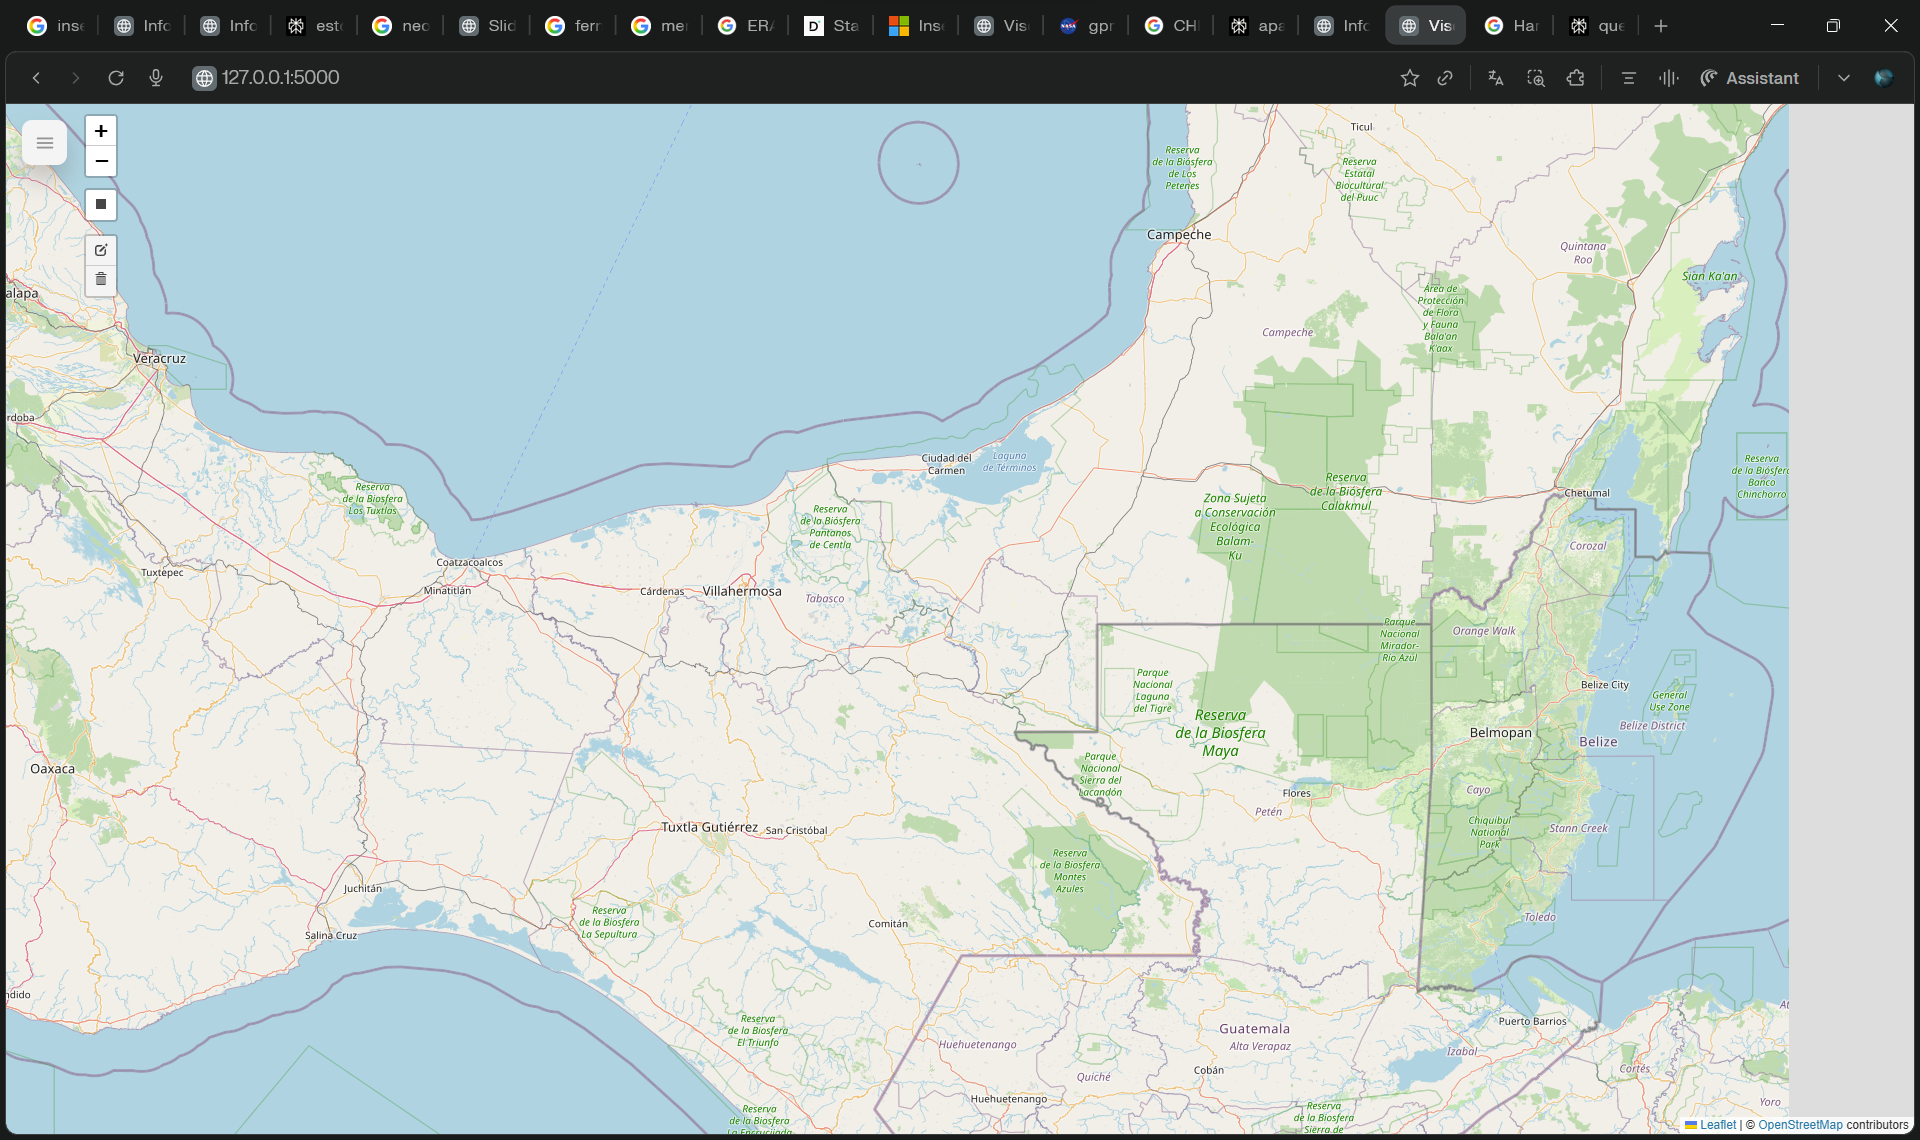
\includegraphics{01-aplicacion-completa.png}}

\end{center}

\vspace{0.3cm}

\begin{itemize}

\item Aplicación web interactiva para visualización geoespacial

\item Análisis de variables meteorológicas y de vegetación

\item Generación de animaciones temporales

\end{itemize}

\end{frame}


\begin{frame}{Flujo de la aplicacion}
\begin{center}

% IMAGEN: Diagrama conceptual simple mostrando: Usuario -> Aplicación Web -> Google Earth Engine -> Visualización

% Puede ser un diagrama de flujo simple con flechas

\resizebox{0.15\textwidth}{!}{
\begin{tikzpicture}[
  node distance=1.8cm,
  every node/.style={rectangle, draw, rounded corners,
                     minimum width=6cm, minimum height=1.1cm,
                     align=center},
  arrow/.style={-Latex, thick}
]

\node (p1) {1. Usuario selecciona área y fechas};
\node[below=of p1] (p2) {2. Frontend envía petición a Flask};
\node[below=of p2] (p3) {3. Flask consulta Earth Engine};
\node[below=of p3] (p4) {4. Earth Engine procesa y genera GIF};
\node[below=of p4] (p5) {5. Respuesta con URL del GIF};
\node[below=of p5] (p6) {6. Frontend muestra resultado};

\draw[arrow] (p1) -- (p2);
\draw[arrow] (p2) -- (p3);
\draw[arrow] (p3) -- (p4);
\draw[arrow] (p4) -- (p5);
\draw[arrow] (p5) -- (p6);

\end{tikzpicture}
}

\end{center}

\end{frame}



% ============================================

% SECCIÓN 3: TECNOLOGÍAS

% ============================================

\section{Tecnologías Utilizadas}



\begin{frame}{Stack Tecnológico}

\begin{center}

% IMAGEN: Logo collage o diagrama con los logos de:

% - Python/Flask

% - Google Earth Engine

% - Leaflet

% - TypeScript

% - HTML5/CSS3

\resizebox{0.4\textwidth}{!}{
\includegraphics{04-stack-tecnologico.png}}

\end{center}

\end{frame}



\begin{frame}{Backend: Flask}

\begin{columns}

\column{0.45\textwidth}

% IMAGEN: Logo de Flask o código Python mostrando estructura básica

\resizebox{0.65\textwidth}{!}{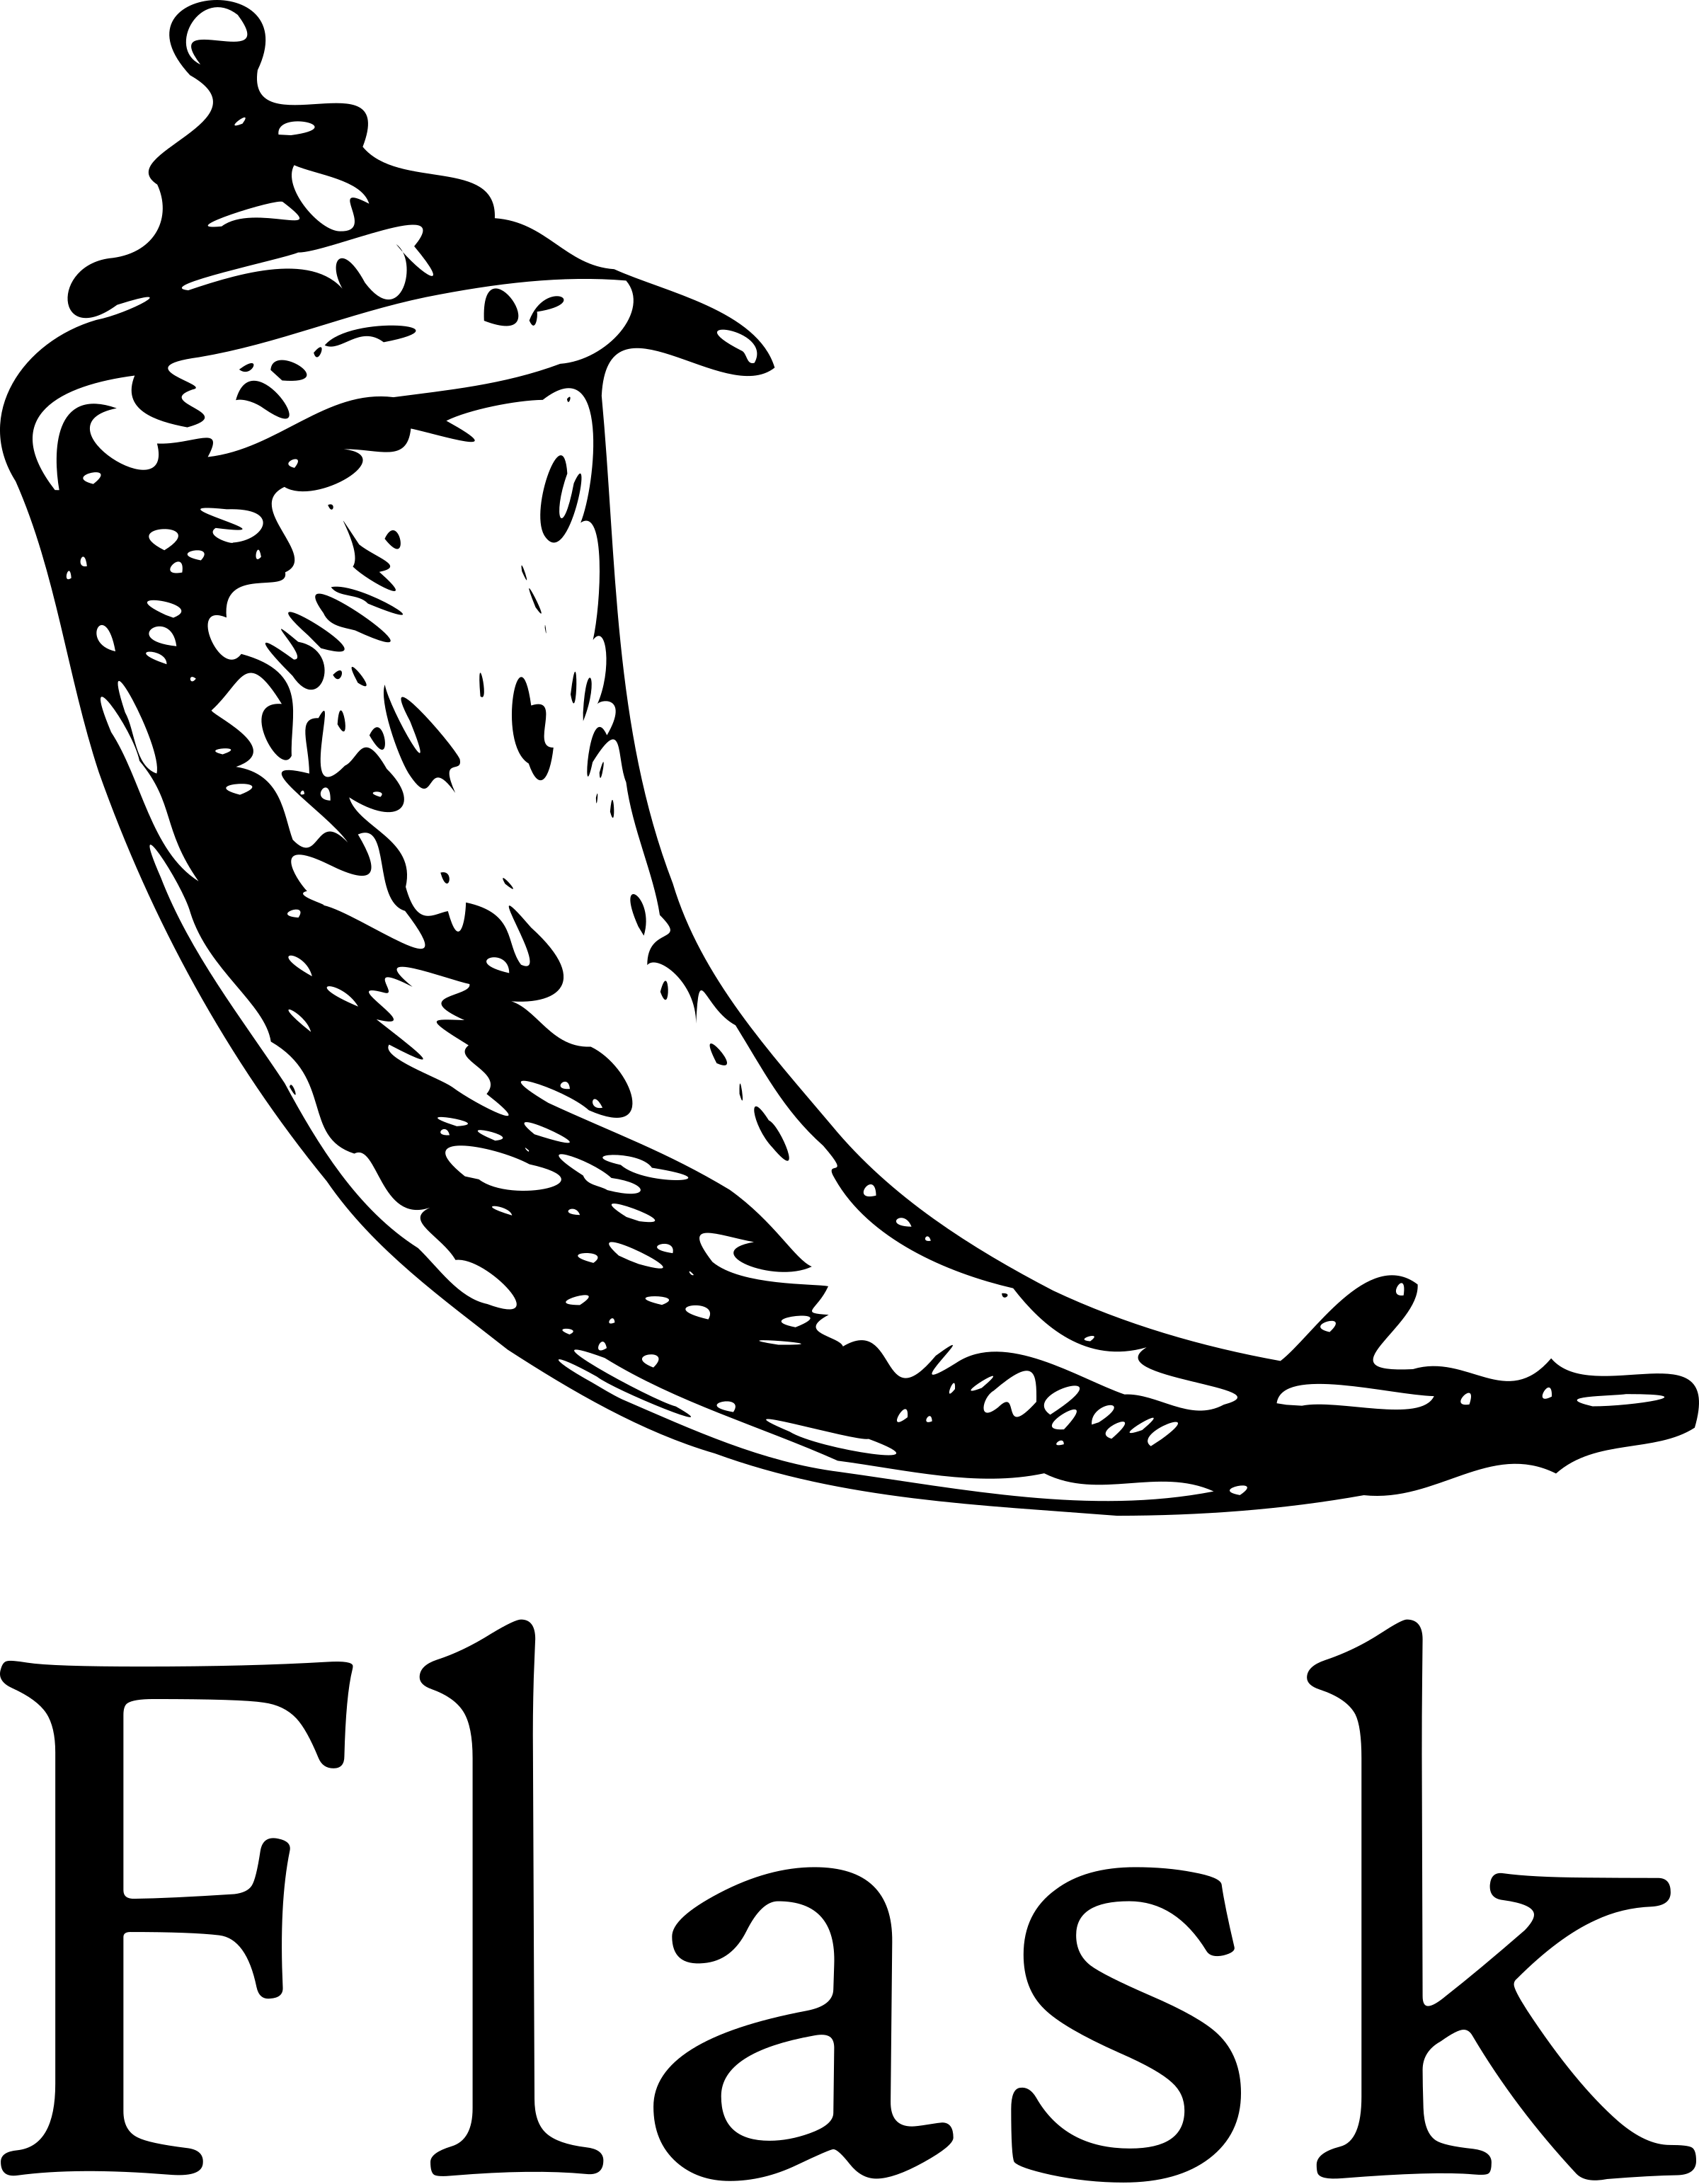
\includegraphics{05-flask.png}}

\column{0.5\textwidth}

\begin{itemize}

\item Framework web minimalista

\item API REST para comunicación

\item Integración con Earth Engine

\item Procesamiento de datos geoespaciales

\end{itemize}

\end{columns}

\end{frame}



\begin{frame}{Procesamiento: Google Earth Engine}

\begin{center}

% IMAGEN: Logo de Google Earth Engine o captura de la plataforma

% Mostrar el poder de procesamiento en la nube

\resizebox{0.55\textwidth}{!}{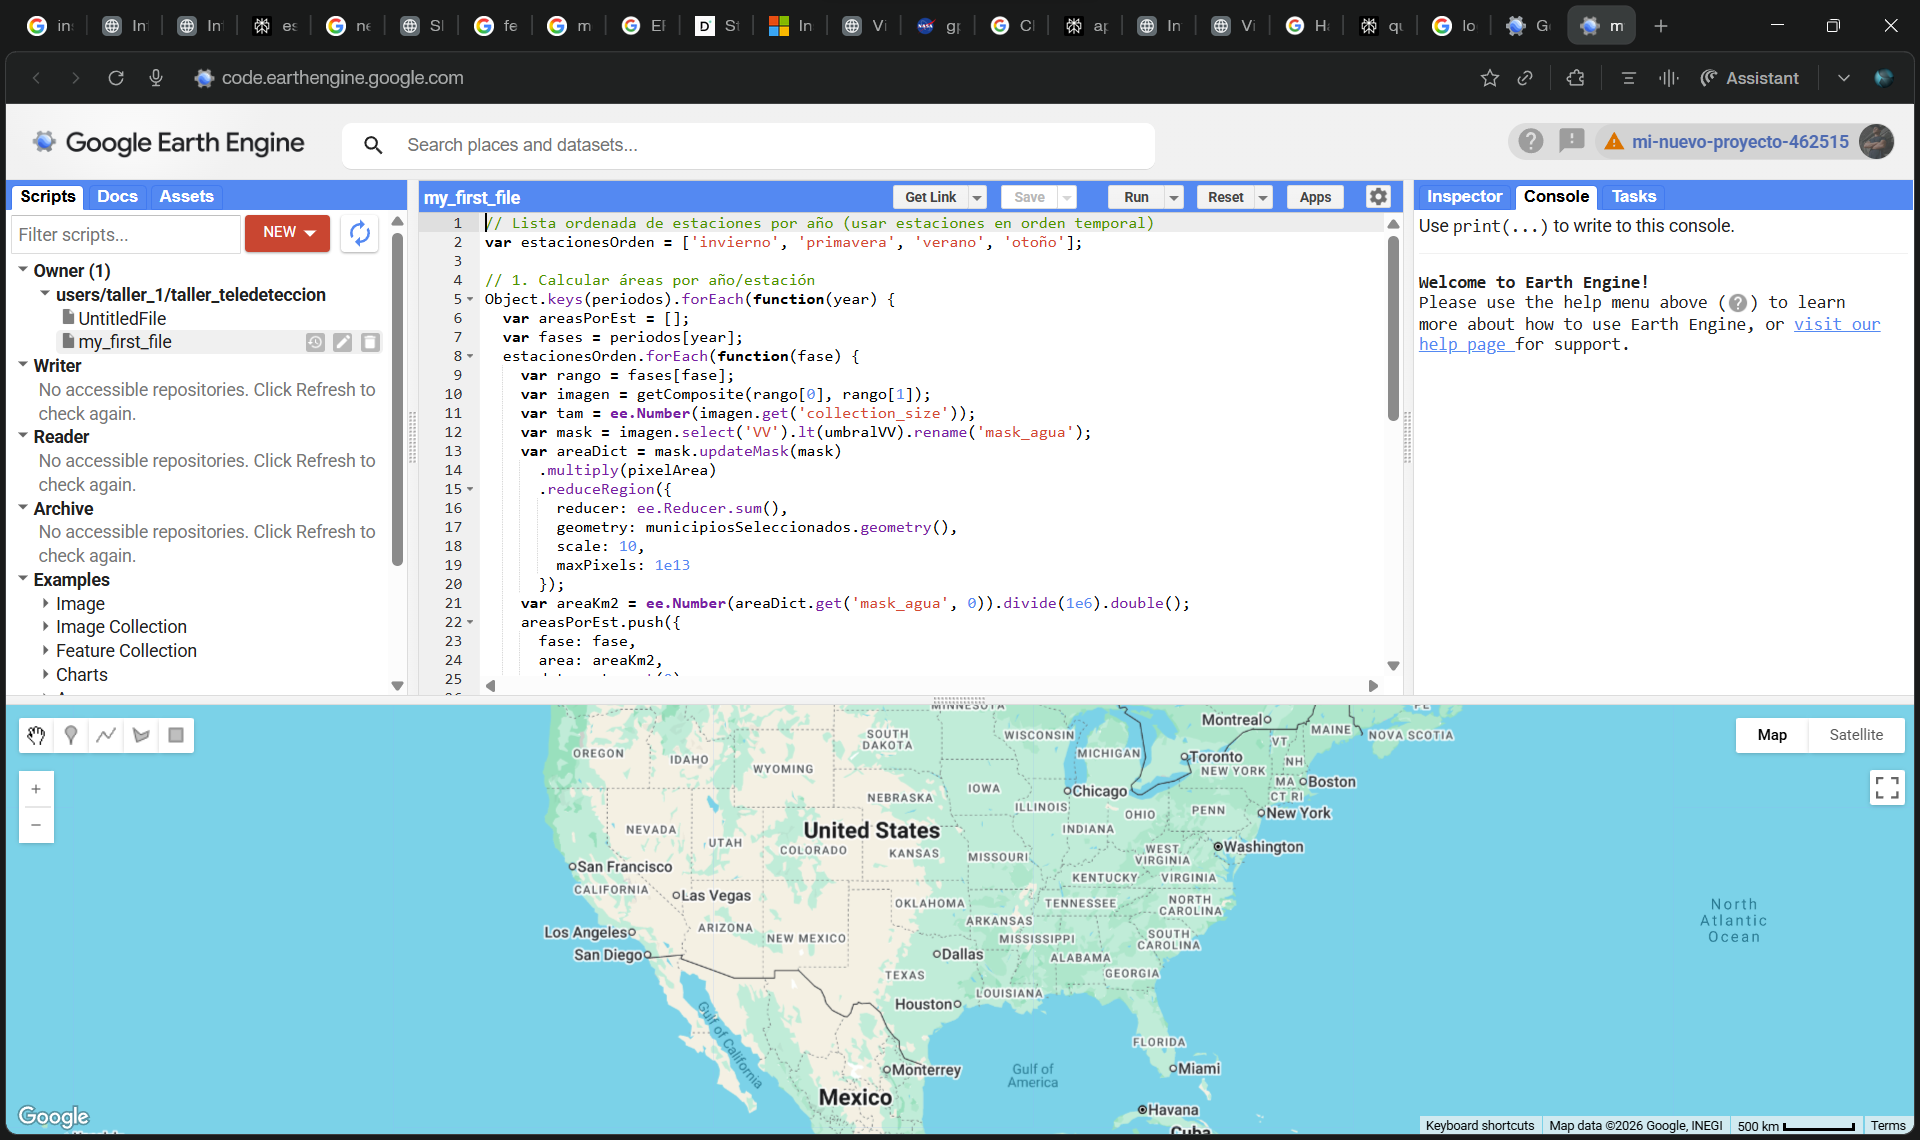
\includegraphics{06-earth-engine.png}}

\end{center}

\vspace{0.3cm}

\begin{itemize}

\item Procesamiento en la nube

\item Acceso a petabytes de datos satelitales

\item Generación de animaciones GIF

\item Cálculo de series temporales

\end{itemize}

\end{frame}



\begin{frame}{Frontend: Leaflet + TypeScript}

\begin{columns}

\column{0.5\textwidth}

% IMAGEN: Captura del mapa interactivo con controles de dibujo visibles

\resizebox{0.9\textwidth}{!}{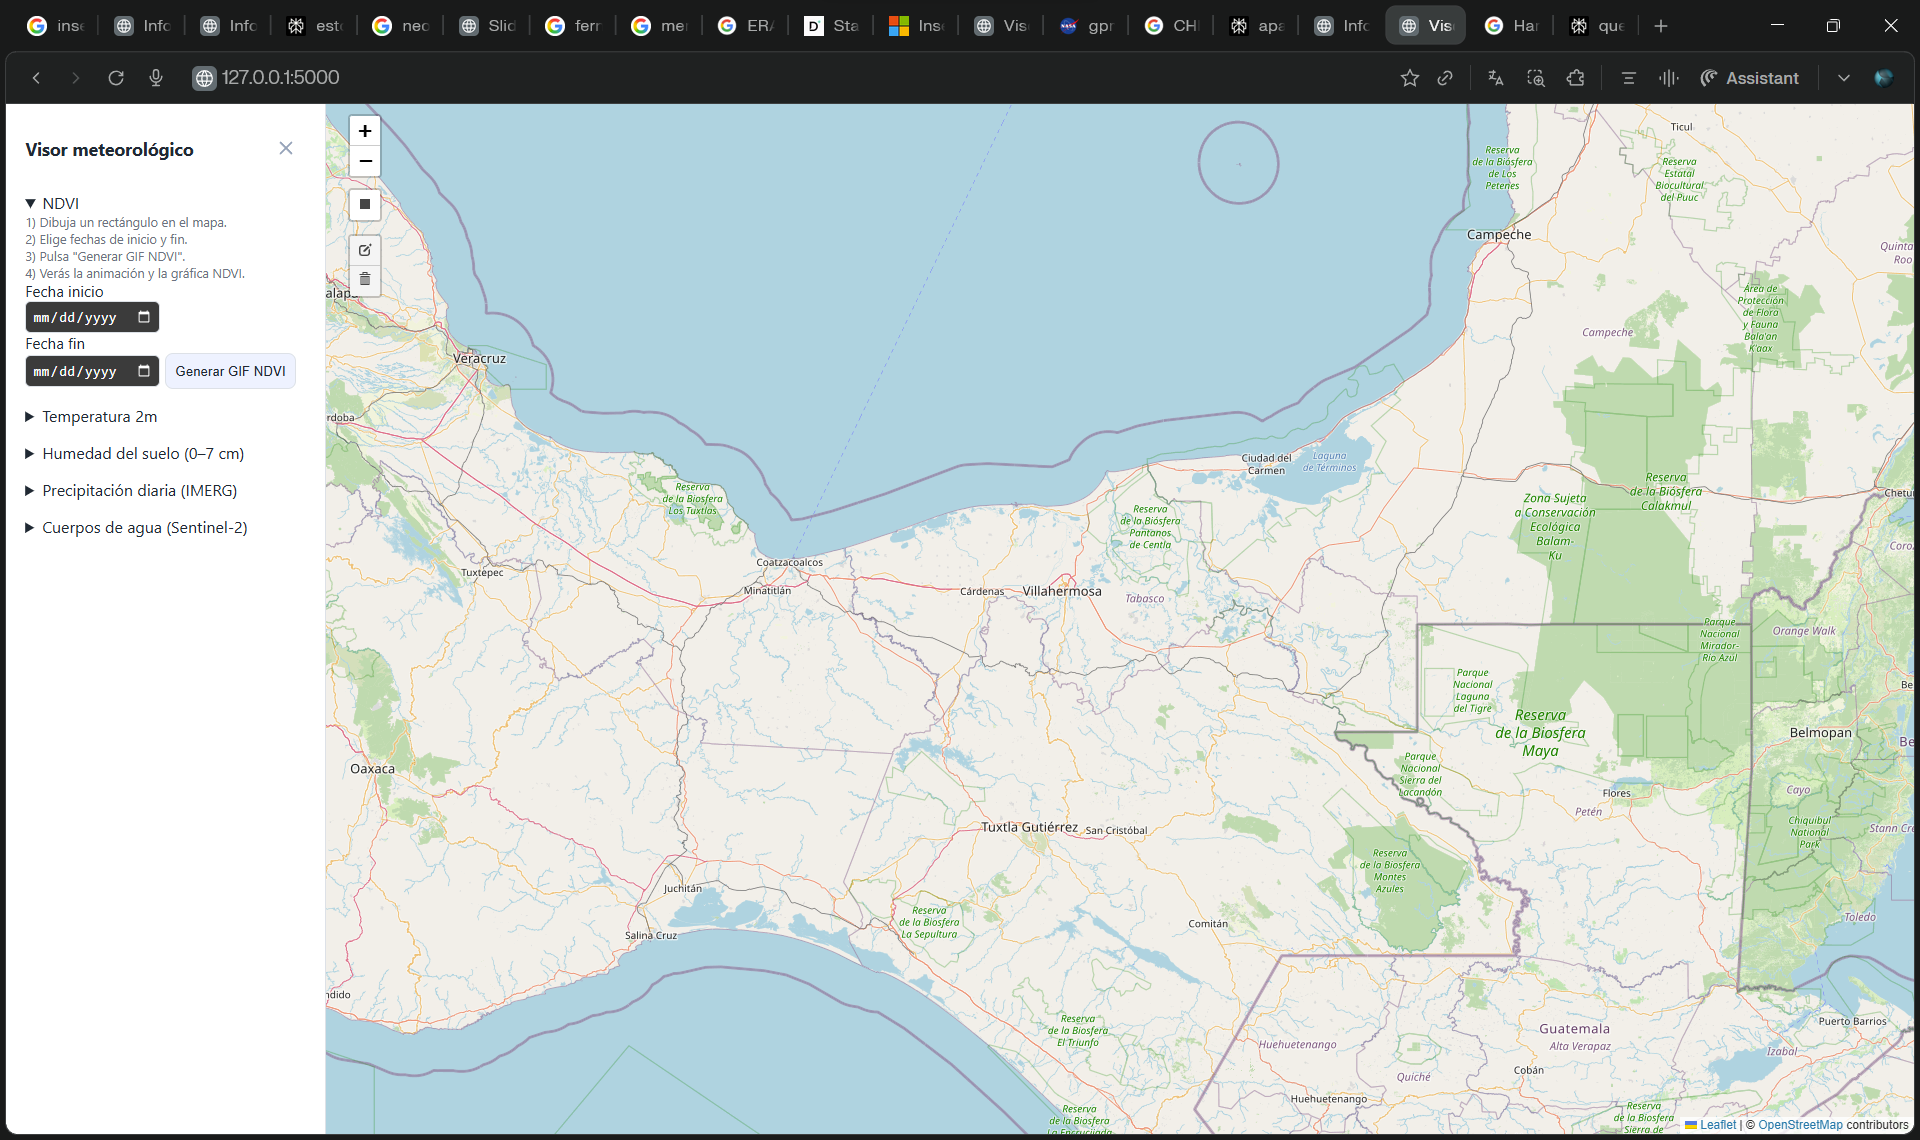
\includegraphics{07-mapa-leaflet.png}}

\column{0.5\textwidth}

\begin{itemize}

\item Mapas interactivos

\item Selección de áreas (bounding boxes)

\item Visualización de overlays

\item Gráficas con Plotly.js

\end{itemize}

\end{columns}

\end{frame}



% ============================================

% SECCIÓN 4: FUNCIONALIDADES

% ============================================

\section{Funcionalidades}

\begin{frame}{Variables Disponibles}

\begin{center}

\only<1>{\textbf{Las variables disponibles son:}}\\

\only<2>{\resizebox{0.5\textwidth}{!}{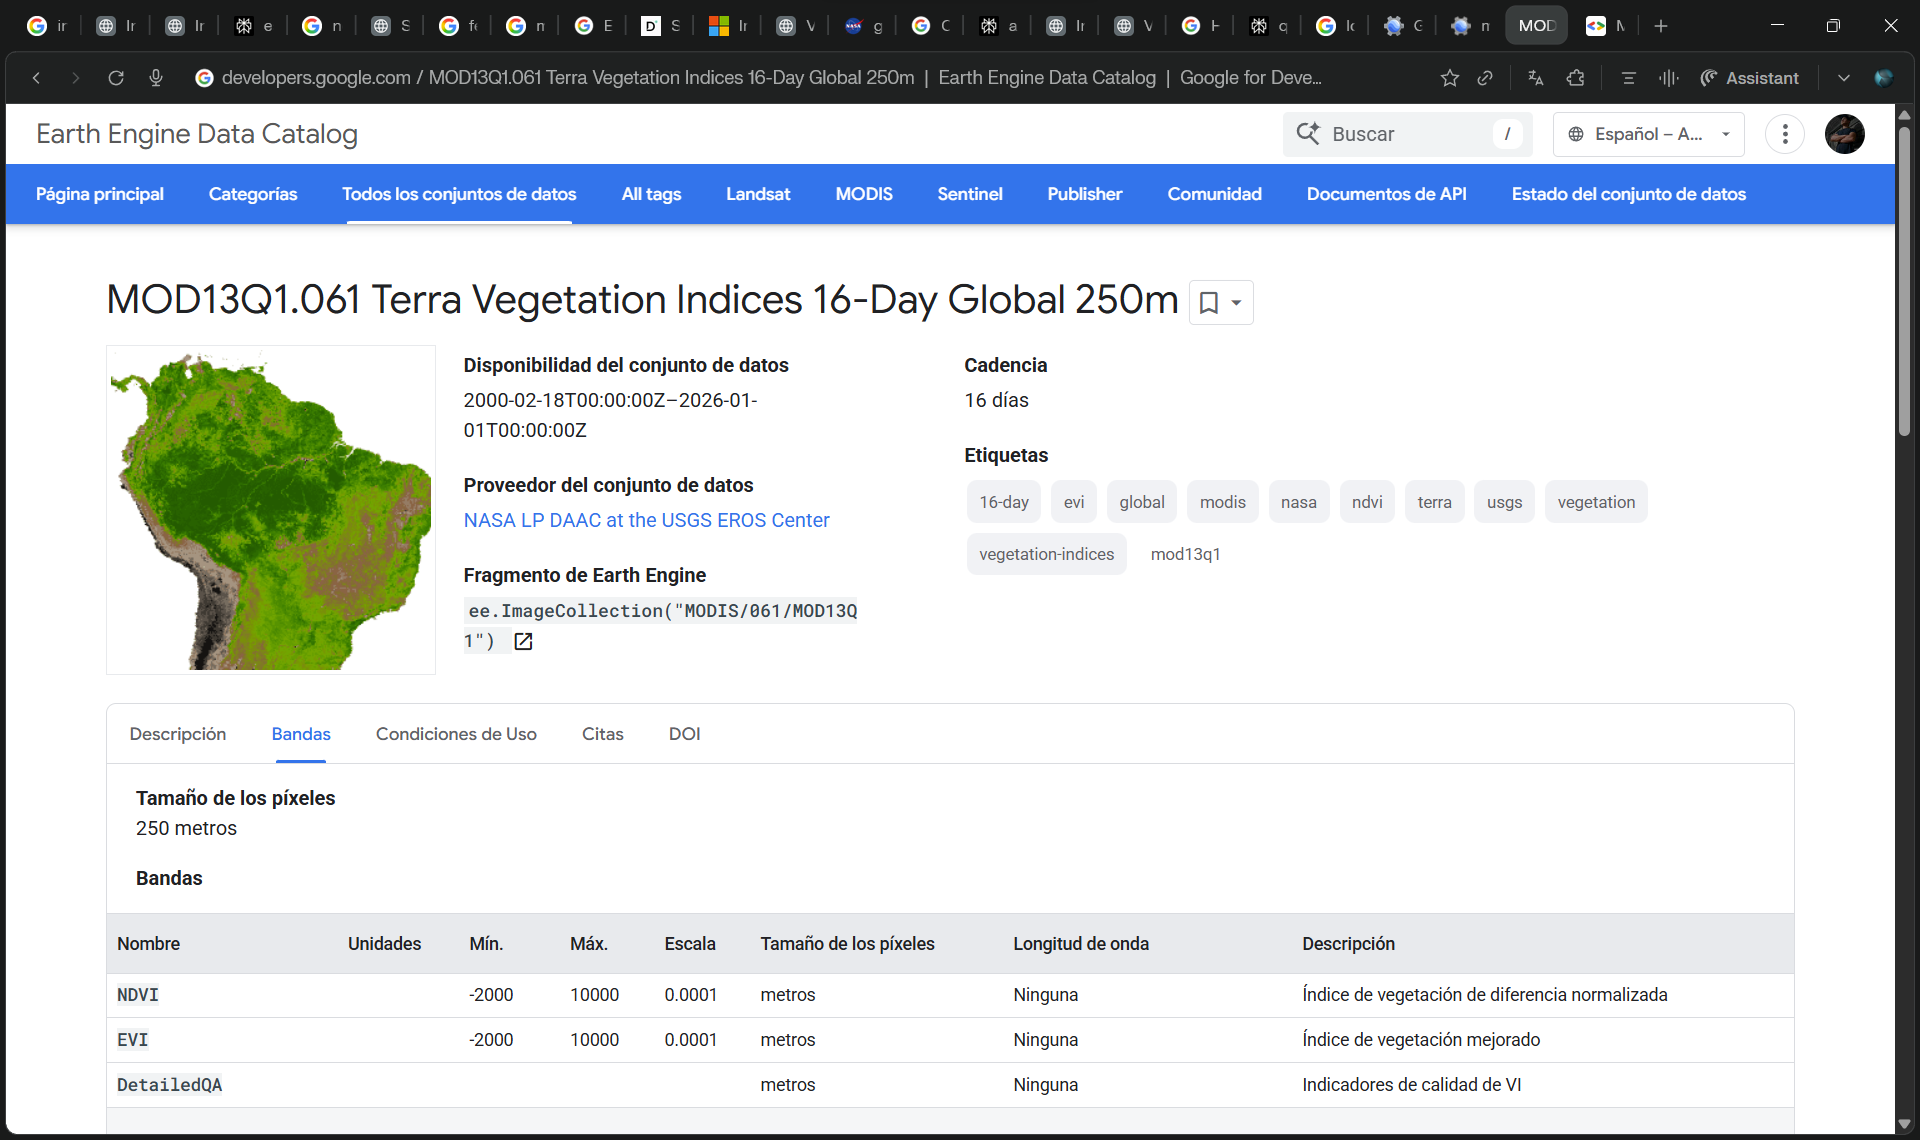
\includegraphics{08a-ndvi.png}}}\\

\only<3>{\resizebox{0.5\textwidth}{!}{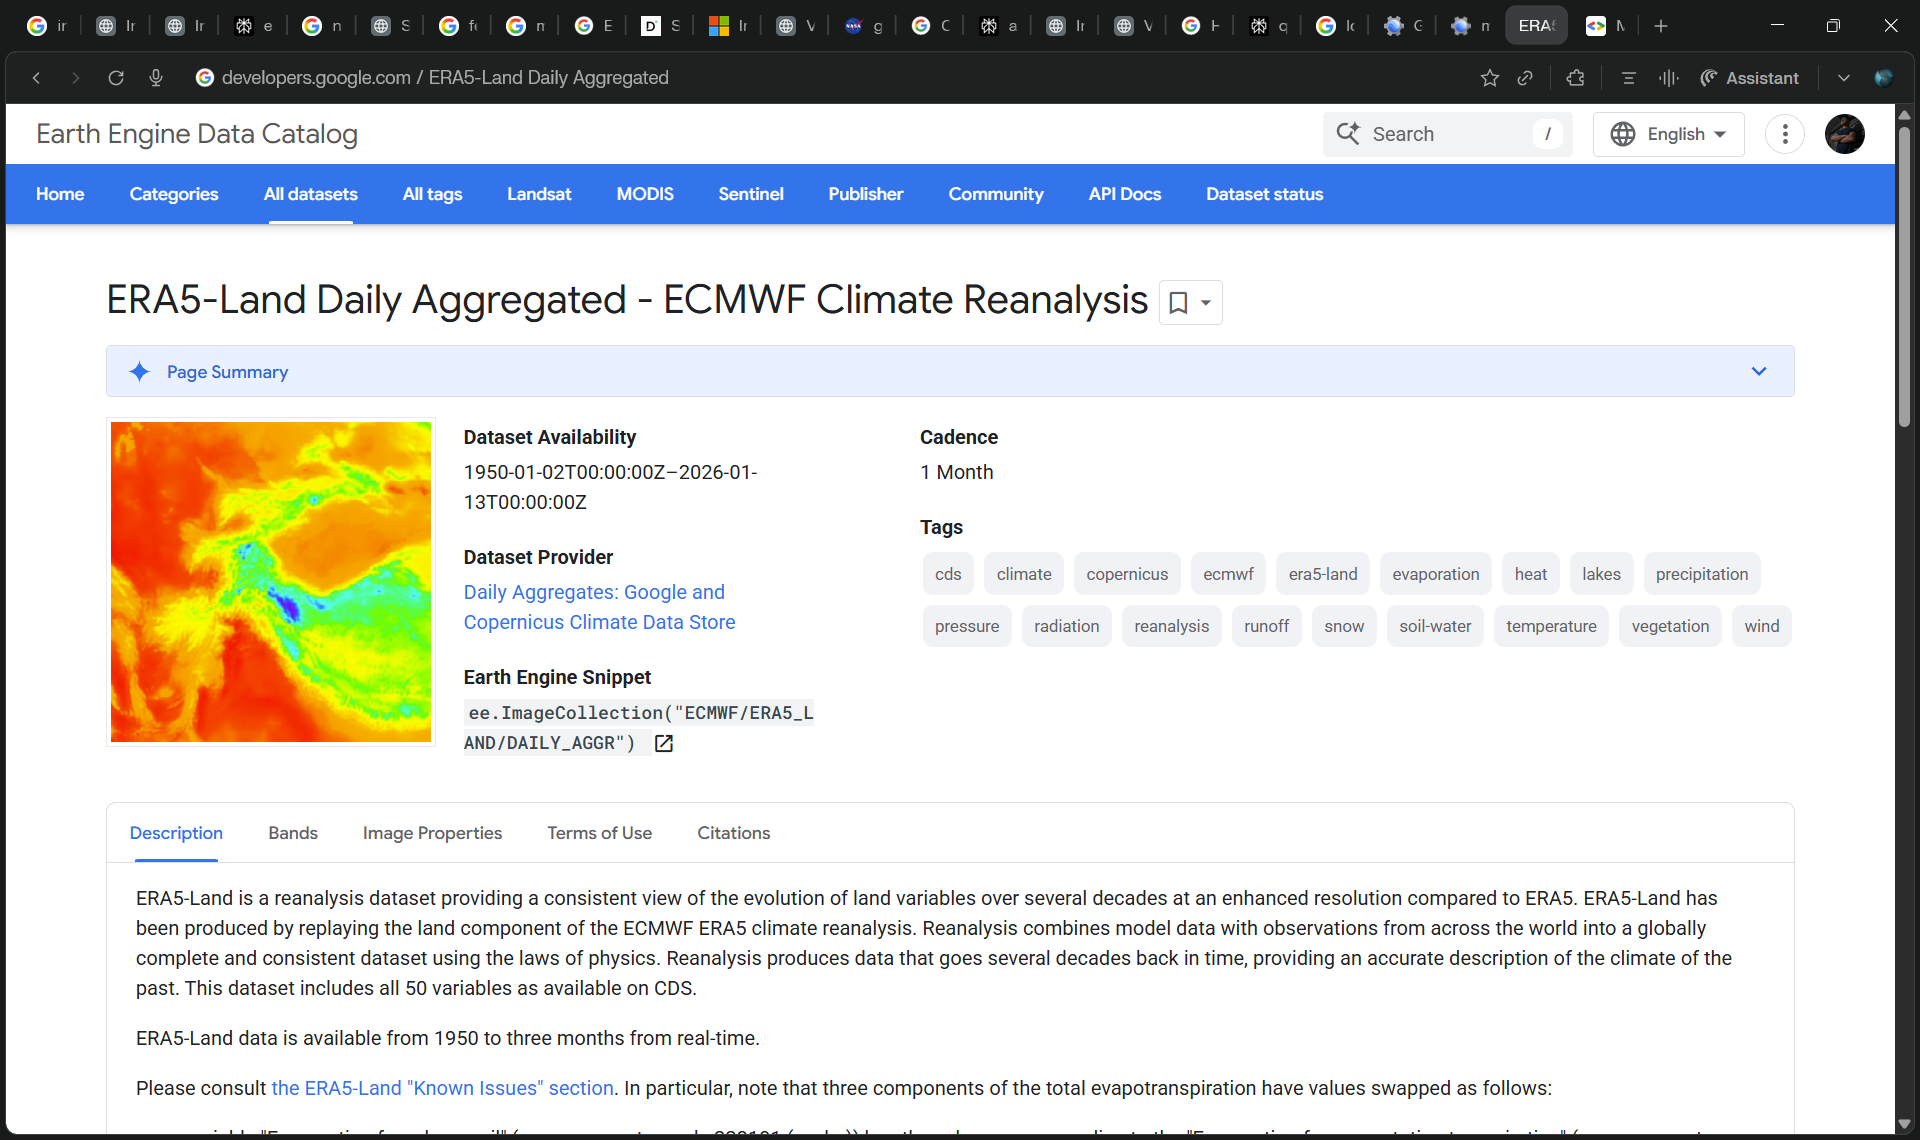
\includegraphics{08b-temperatura.png}}}\\

\only<4>{\resizebox{0.5\textwidth}{!}{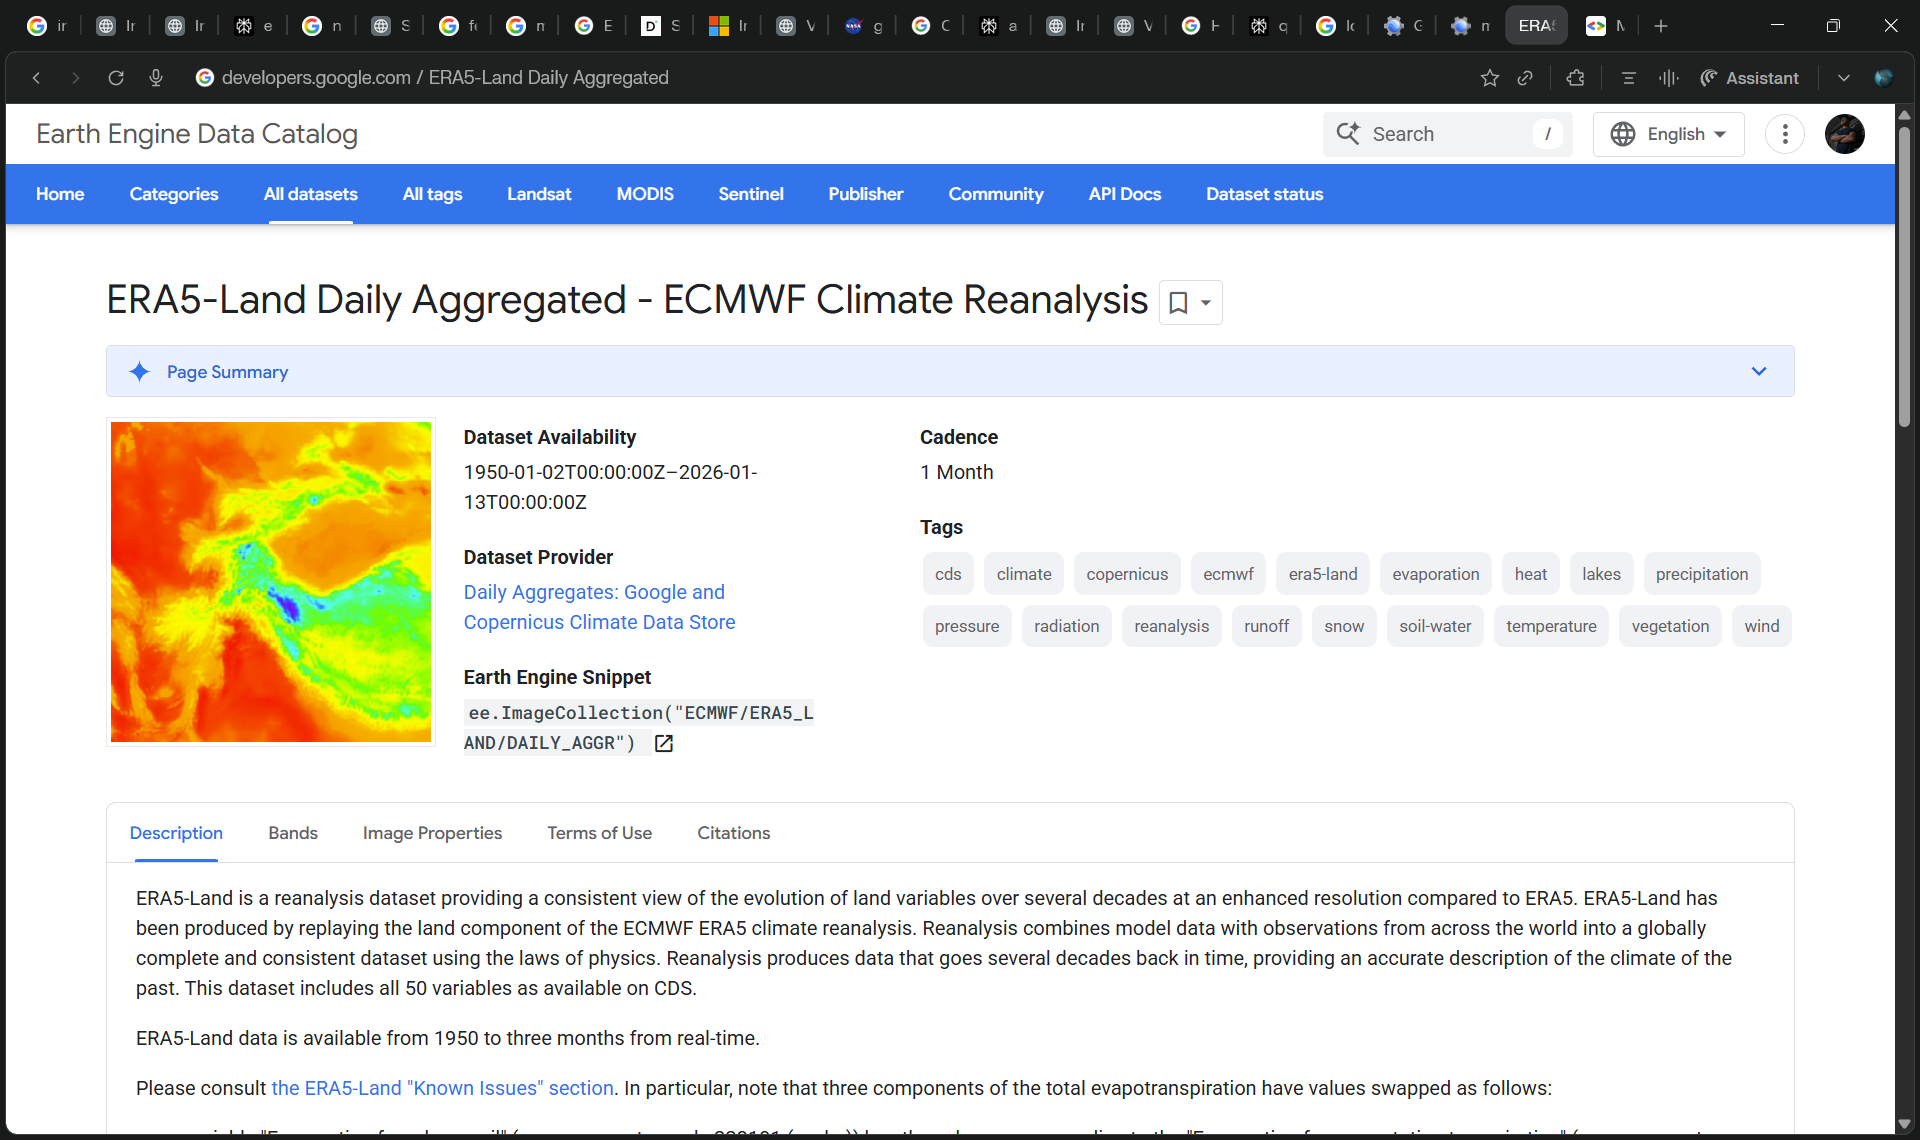
\includegraphics{08c-humedad-suelo.png}}}\\

\only<5>{\resizebox{0.5\textwidth}{!}{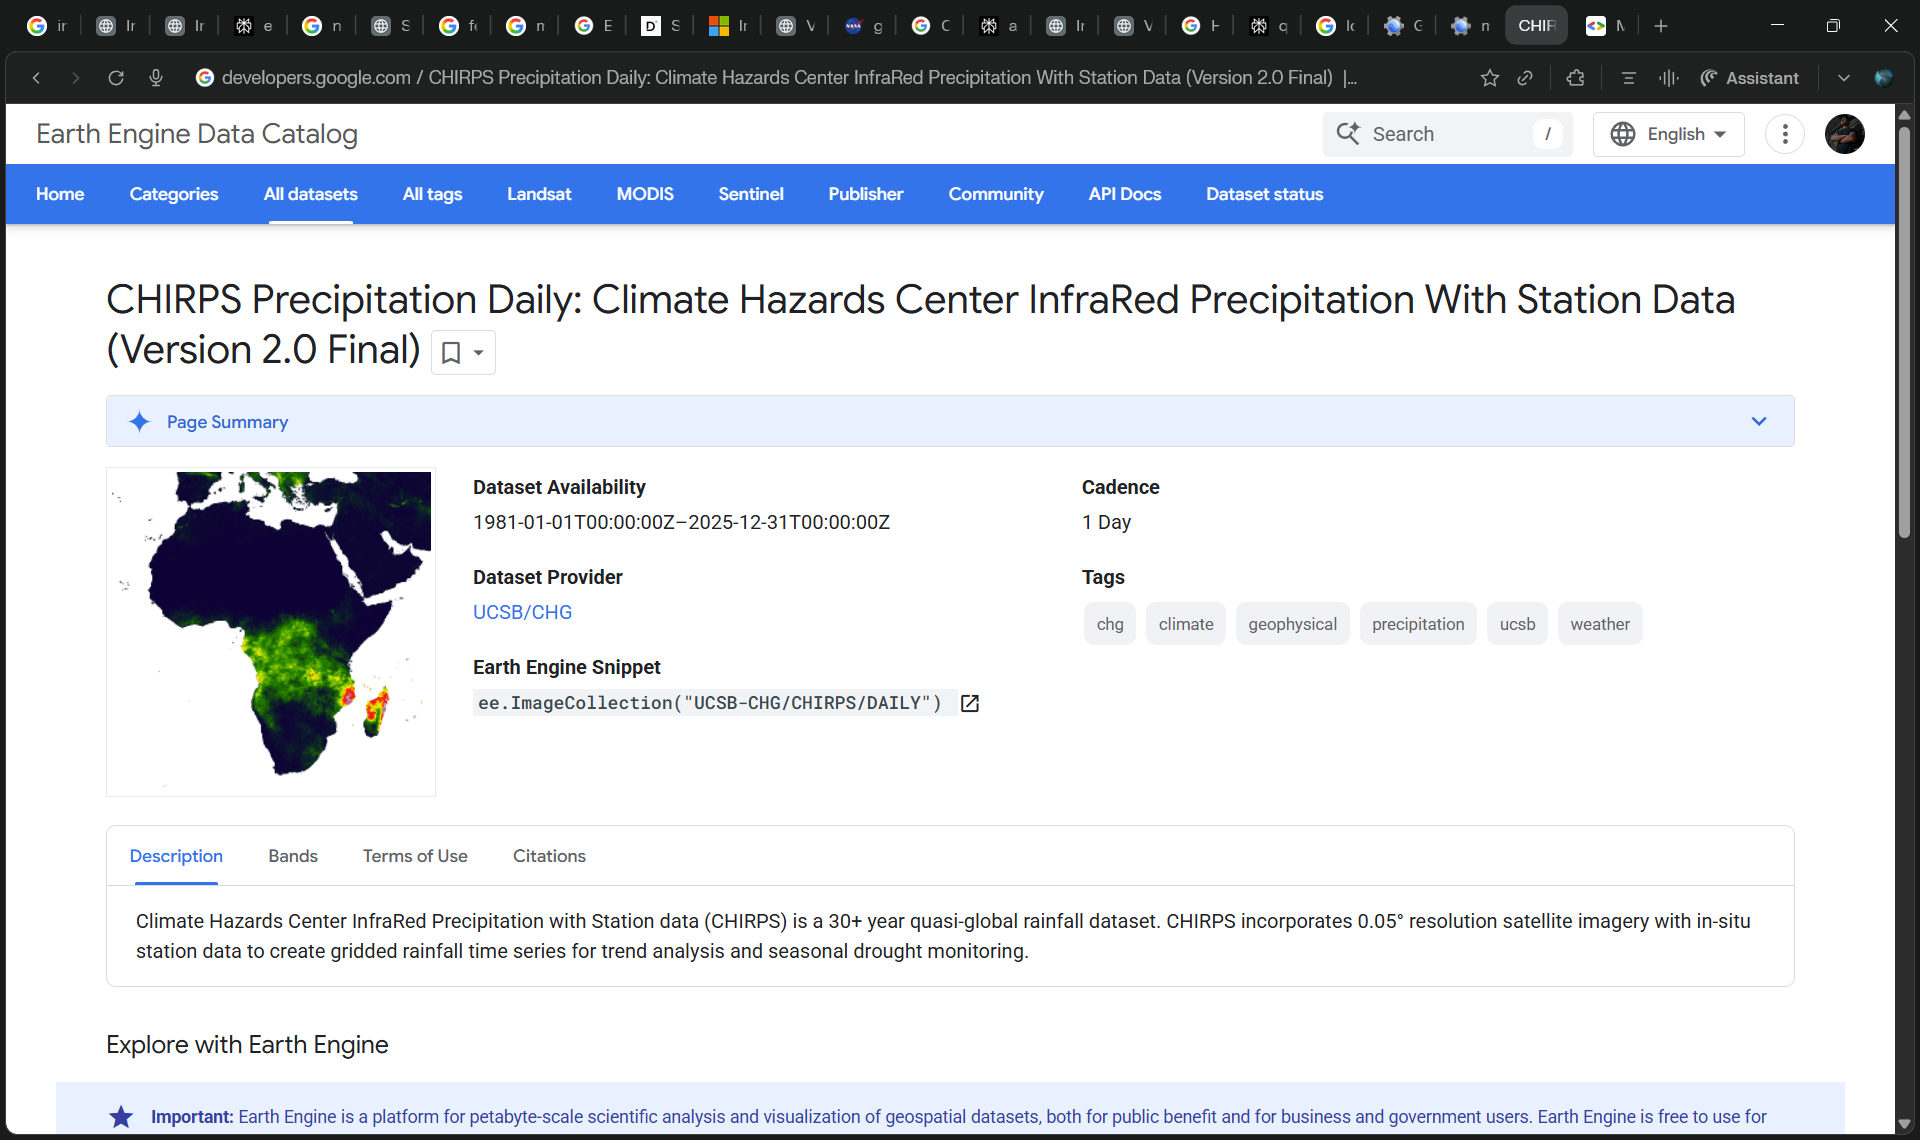
\includegraphics{08d-precipitacion.png}}}\\

\only<6>{\resizebox{0.5\textwidth}{!}{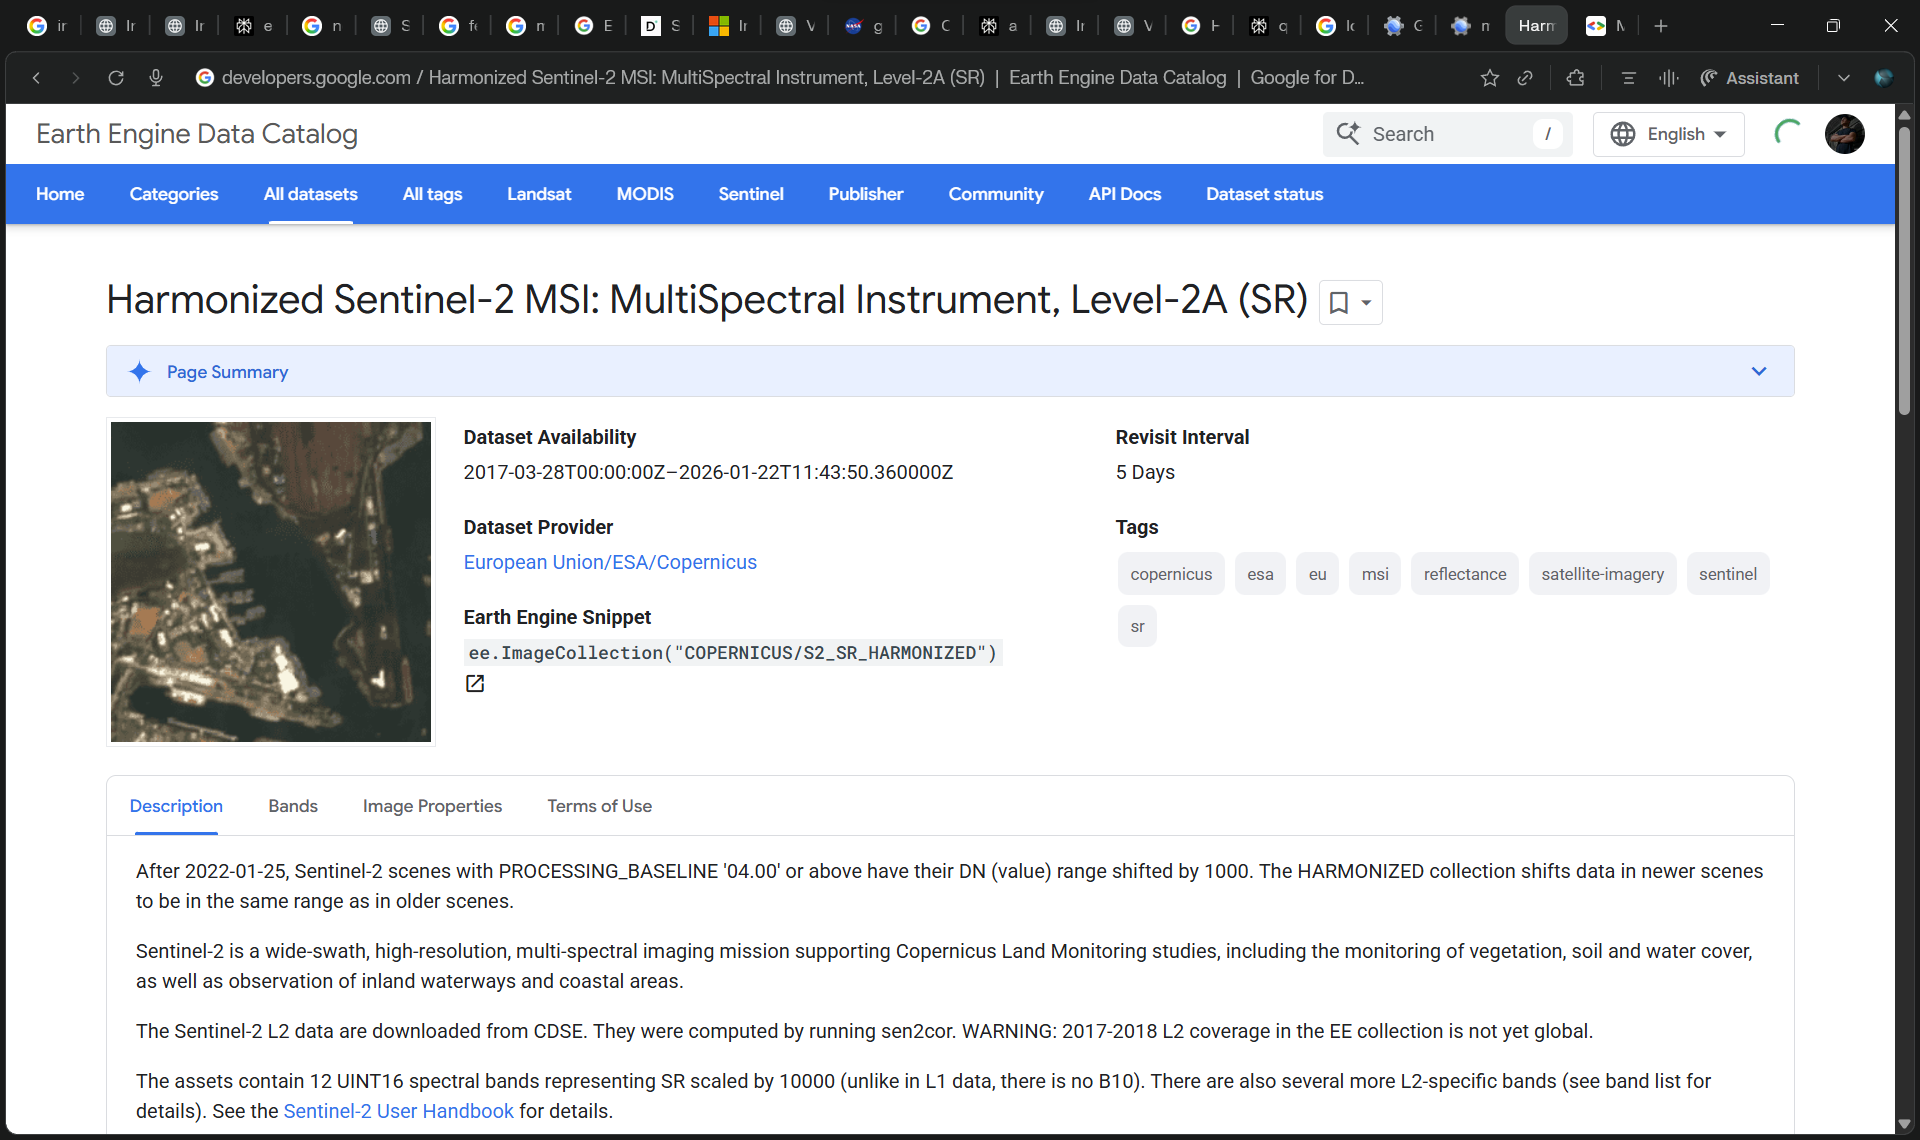
\includegraphics{08e-agua-superficial.png}}}

\end{center}

\vspace{0.2cm}

\begin{itemize}

\item<only@2> \textbf{NDVI (MODIS MOD13Q1)}: Índice de Vegetación de Diferencia Normalizada,\\
refleja la salud y densidad de la vegetación (250m, 16 días).

\item<only@3> \textbf{Temperatura 2m (ERA5-Land Daily)}: Temperatura del aire a 2 metros,\\
datos de reanálisis global convertidos a Celsius ($\sim$11 km, diaria).

\item<only@4> \textbf{Humedad del Suelo (ERA5-Land, 0-7cm)}: Porcentaje volumétrico de agua\\
en la capa superficial ($\sim$11 km, diaria).

\item<only@5> \textbf{Precipitación (CHIRPS Daily)}: Estimaciones globales de precipitación\\
combinando satélite y estaciones ($\sim$5.5 km, diaria).

\item<only@6> \textbf{Agua Superficial (Copernicus Sentinel-2, NDWI)}: Mapeo detallado de cuerpos\\
de agua y zonas inundadas (10m, $\sim$5 días).

\end{itemize}

\end{frame}

\begin{frame}{Selección de Área}

\begin{center}

% IMAGEN: Captura del mapa mostrando un rectángulo dibujado

% Mostrar claramente el área seleccionada con el control de dibujo activo

\resizebox{0.55\textwidth}{!}{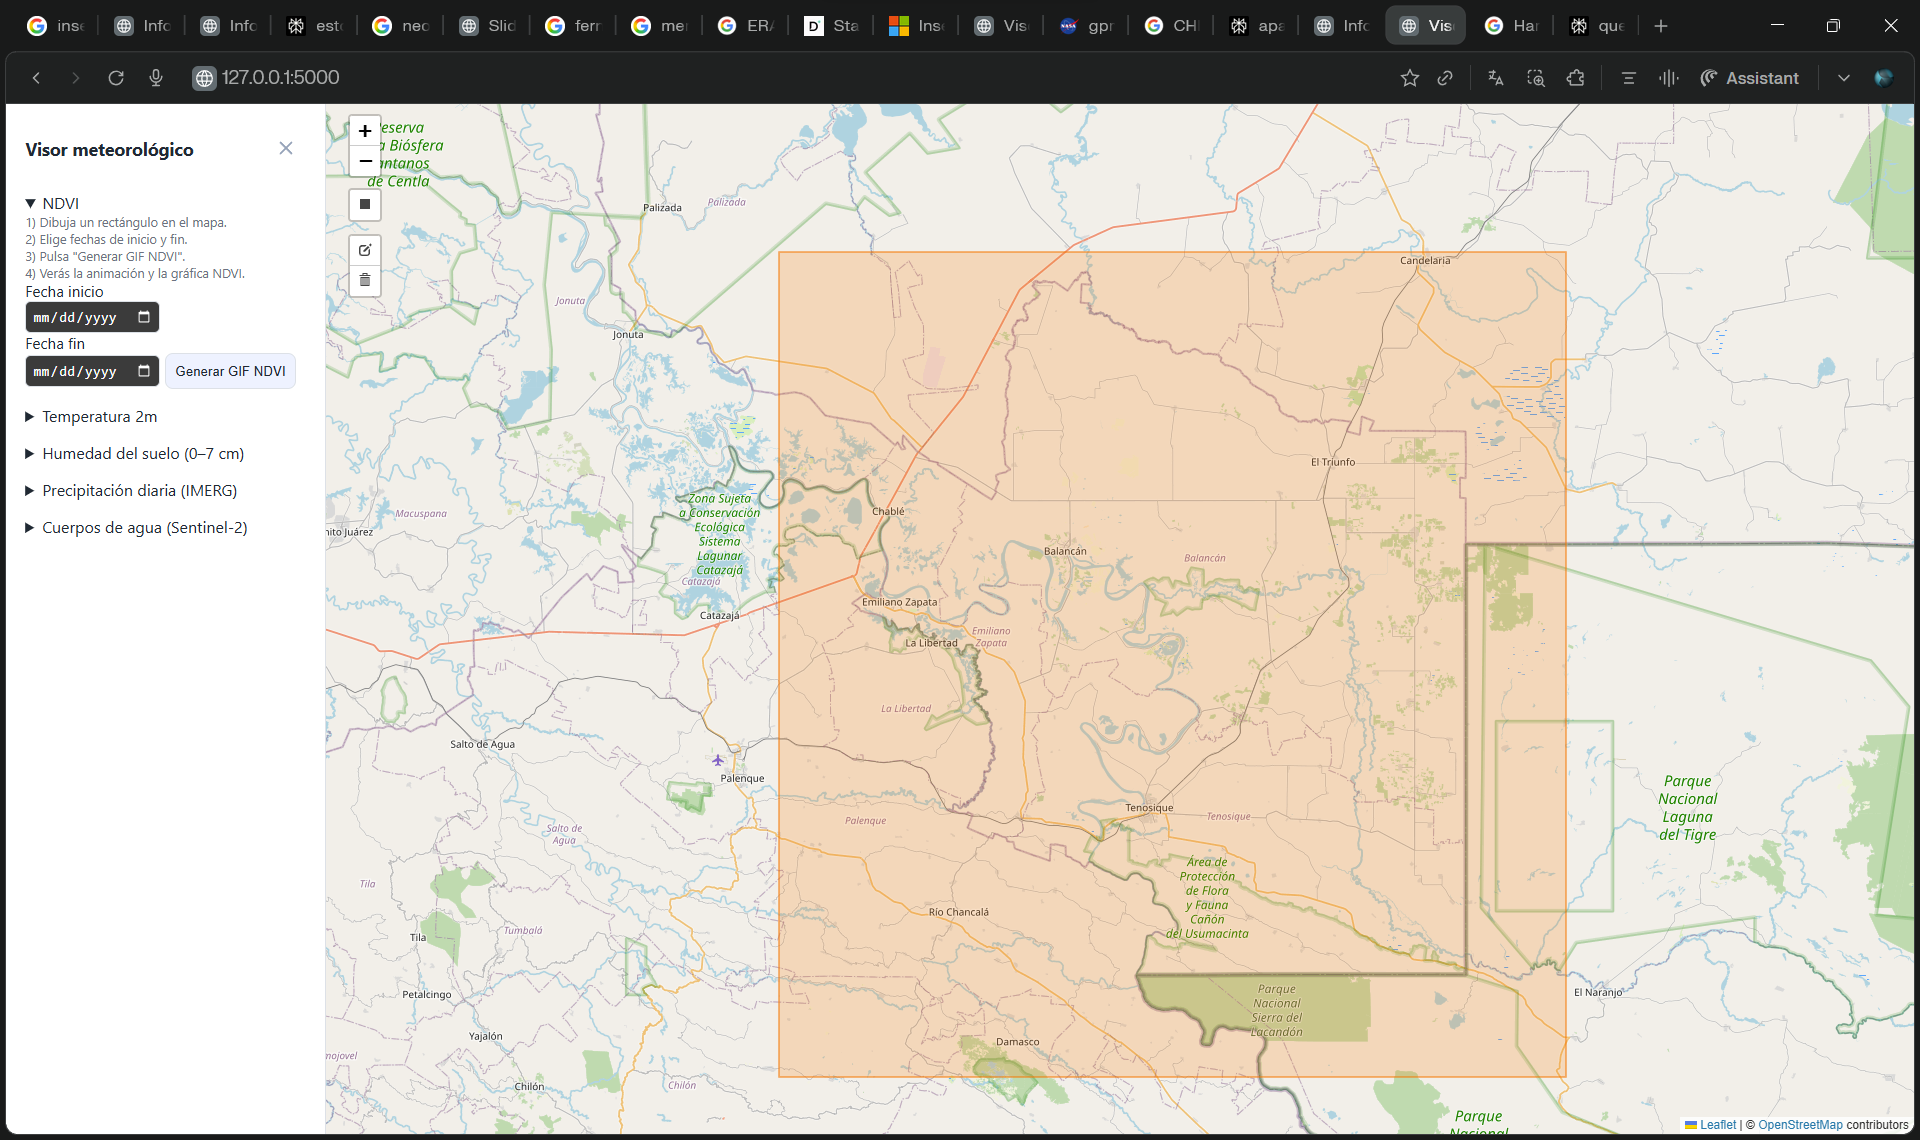
\includegraphics{10-seleccion-area.png}}

\end{center}

\vspace{0.3cm}

\begin{itemize}

\item Herramienta de dibujo integrada

\item Validación de tamaño máximo (8° por lado)

\item Conversión automática a cuadrado

\end{itemize}

\end{frame}



\begin{frame}{Generación de Animaciones}

\begin{center}

% IMAGEN: Captura mostrando un GIF animado de NDVI superpuesto en el mapa

% Mostrar la animación temporal con la barra de colores visible

\resizebox{0.55\textwidth}{!}{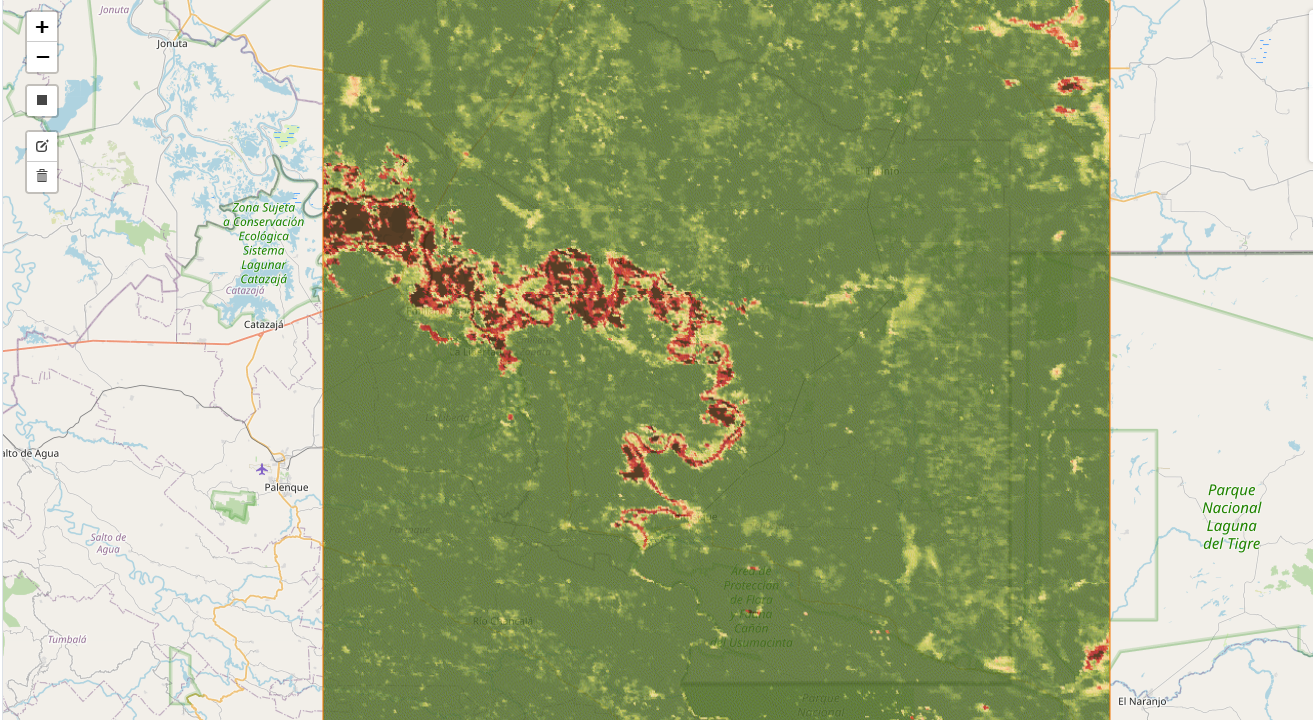
\includegraphics{11-animacion-ndvi.png}}

\end{center}

\vspace{0.2cm}

\begin{itemize}

\item Animaciones GIF temporales

\item Paletas de colores personalizadas

\item Control de resolución automático

\end{itemize}

\end{frame}



\begin{frame}{Series Temporales}

\begin{center}

% IMAGEN: Captura de la gráfica interactiva de Plotly mostrando una serie temporal

% Mostrar la gráfica con datos de NDVI o temperatura a lo largo del tiempo

\resizebox{0.75\textwidth}{!}{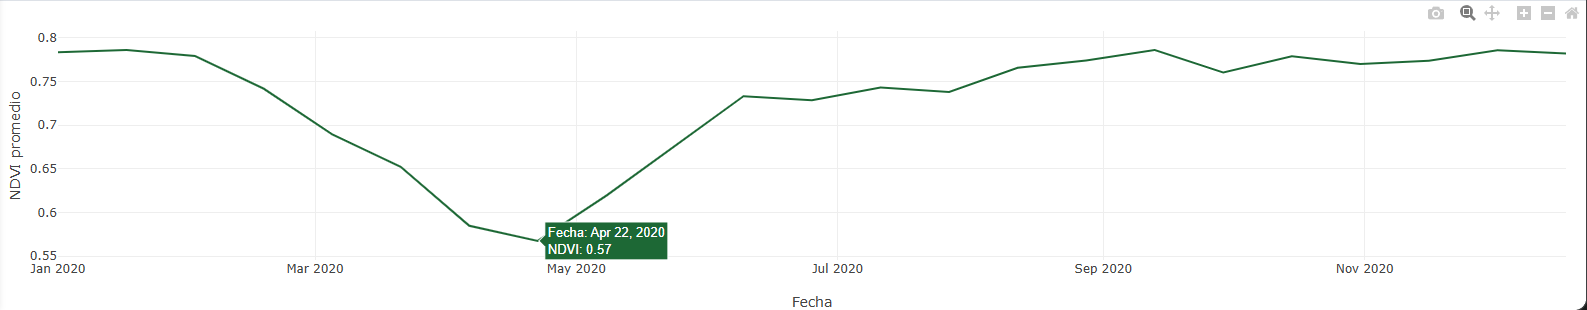
\includegraphics{12-serie-temporal.png}}

\end{center}

\vspace{0.2cm}

\begin{itemize}

\item Gráficas interactivas

\item Zoom y pan

\item Hover con información detallada

\end{itemize}

\end{frame}



% ============================================

% SECCIÓN 5: ARQUITECTURA

% ============================================

\section{Arquitectura}

\begin{frame}{Flujo de Datos}

\begin{center}

\resizebox{0.15\textwidth}{!}{
\begin{tikzpicture}[
  node distance=1.8cm,
  every node/.style={rectangle, draw, rounded corners,
                     minimum width=6cm, minimum height=1.1cm,
                     align=center},
  arrow/.style={-Latex, thick}
]

\node (p1) {1. Usuario selecciona área y fechas};
\node[below=of p1] (p2) {2. Frontend envía petición a Flask};
\node[below=of p2] (p3) {3. Flask consulta Earth Engine};
\node[below=of p3] (p4) {4. Earth Engine procesa y genera GIF};
\node[below=of p4] (p5) {5. Respuesta con URL del GIF};
\node[below=of p5] (p6) {6. Frontend muestra resultado};

\draw[arrow] (p1) -- (p2);
\draw[arrow] (p2) -- (p3);
\draw[arrow] (p3) -- (p4);
\draw[arrow] (p4) -- (p5);
\draw[arrow] (p5) -- (p6);

\end{tikzpicture}
}

\end{center}

\end{frame}

% ============================================

% SECCIÓN 6: FUENTES DE DATOS

% ============================================

\section{Fuentes de Datos}

% ============================================

% SECCIÓN 8: RESULTADOS

% ============================================

\section{Resultados}



\begin{frame}{Ejemplo: Análisis NDVI}

\begin{center}

% IMAGEN: Captura mostrando un análisis completo:

% - GIF de NDVI animado

% - Gráfica de serie temporal

% - Barra de colores visible

\resizebox{0.75\textwidth}{!}{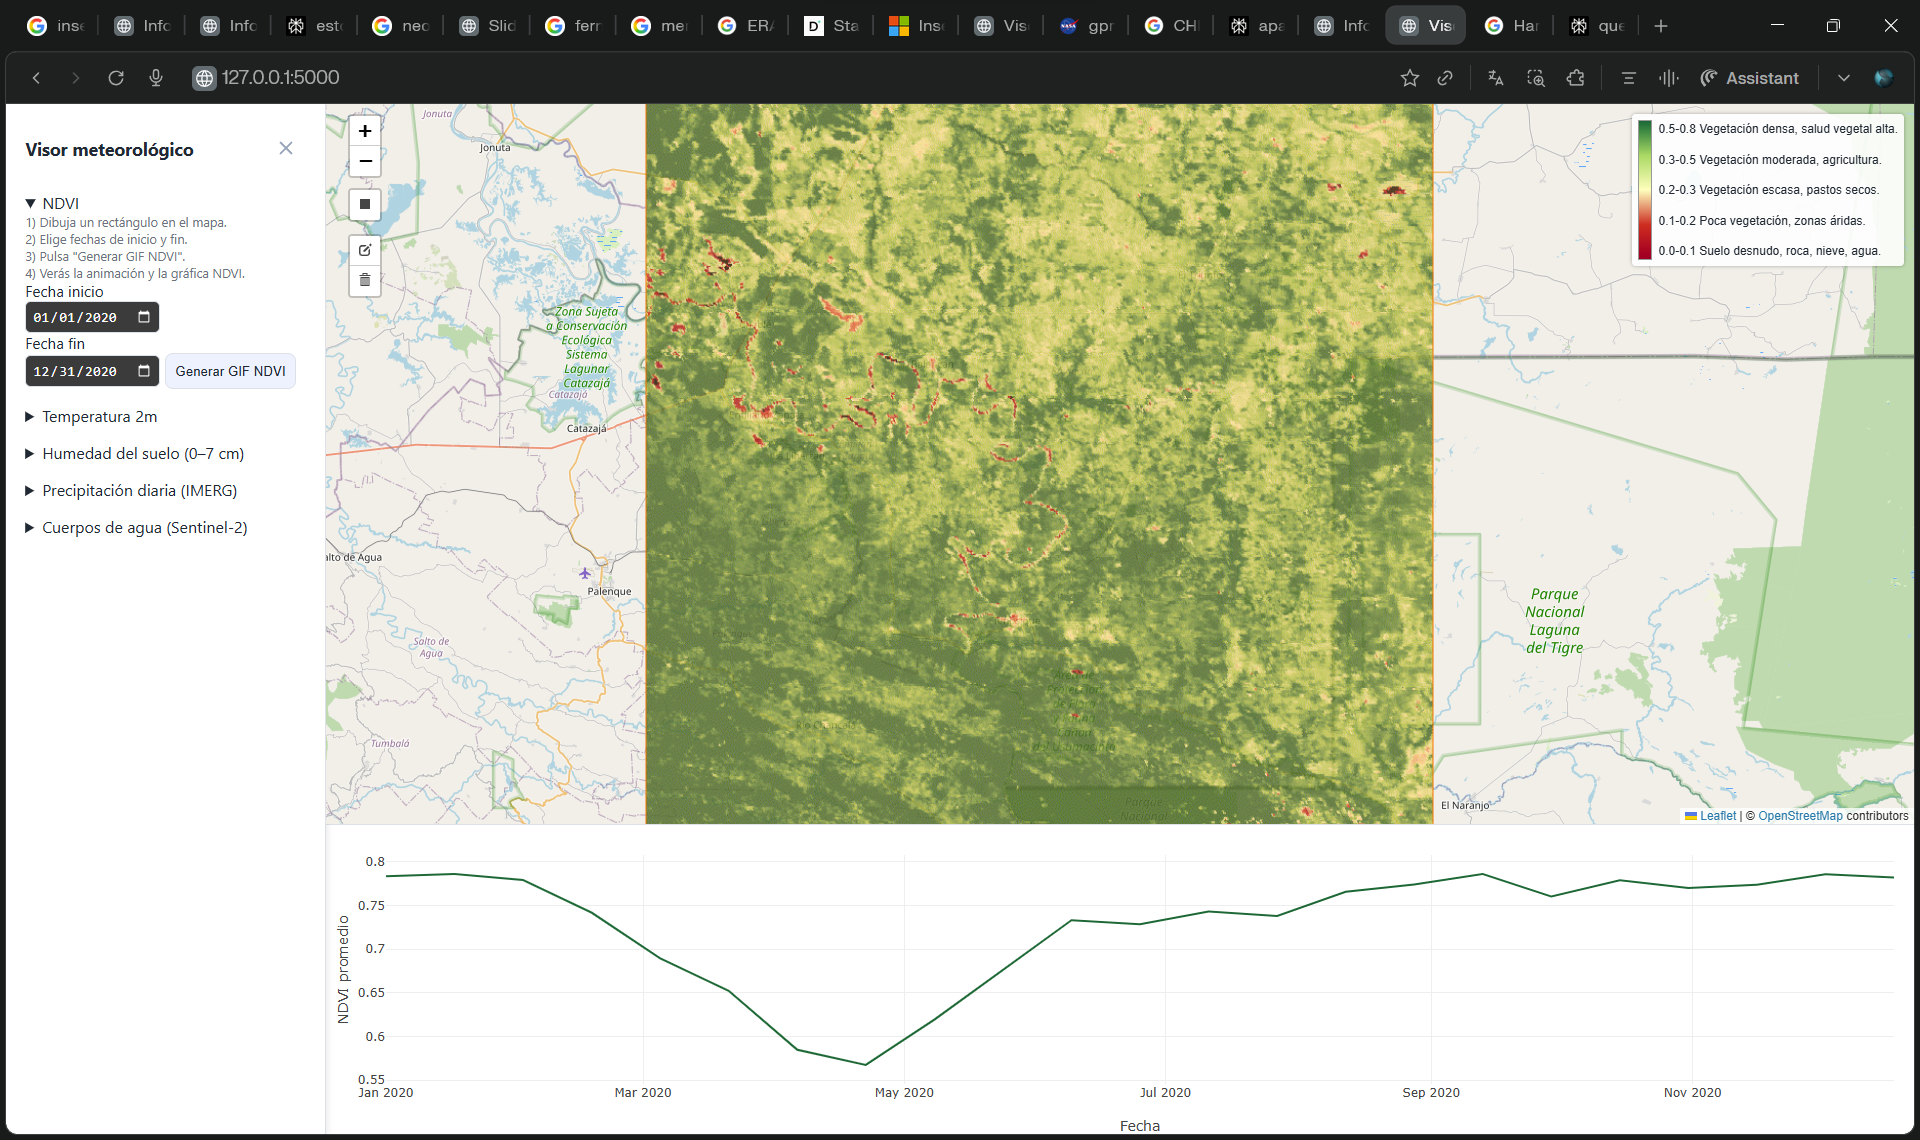
\includegraphics{20-ejemplo-ndvi.png}}

\end{center}

\end{frame}



\begin{frame}{Ejemplo: Análisis de Temperatura}

\begin{center}

% IMAGEN: Captura mostrando análisis de temperatura:

% - GIF de temperatura

% - Gráfica de serie temporal de temperatura

% - Barra de colores de temperatura

\resizebox{0.75\textwidth}{!}{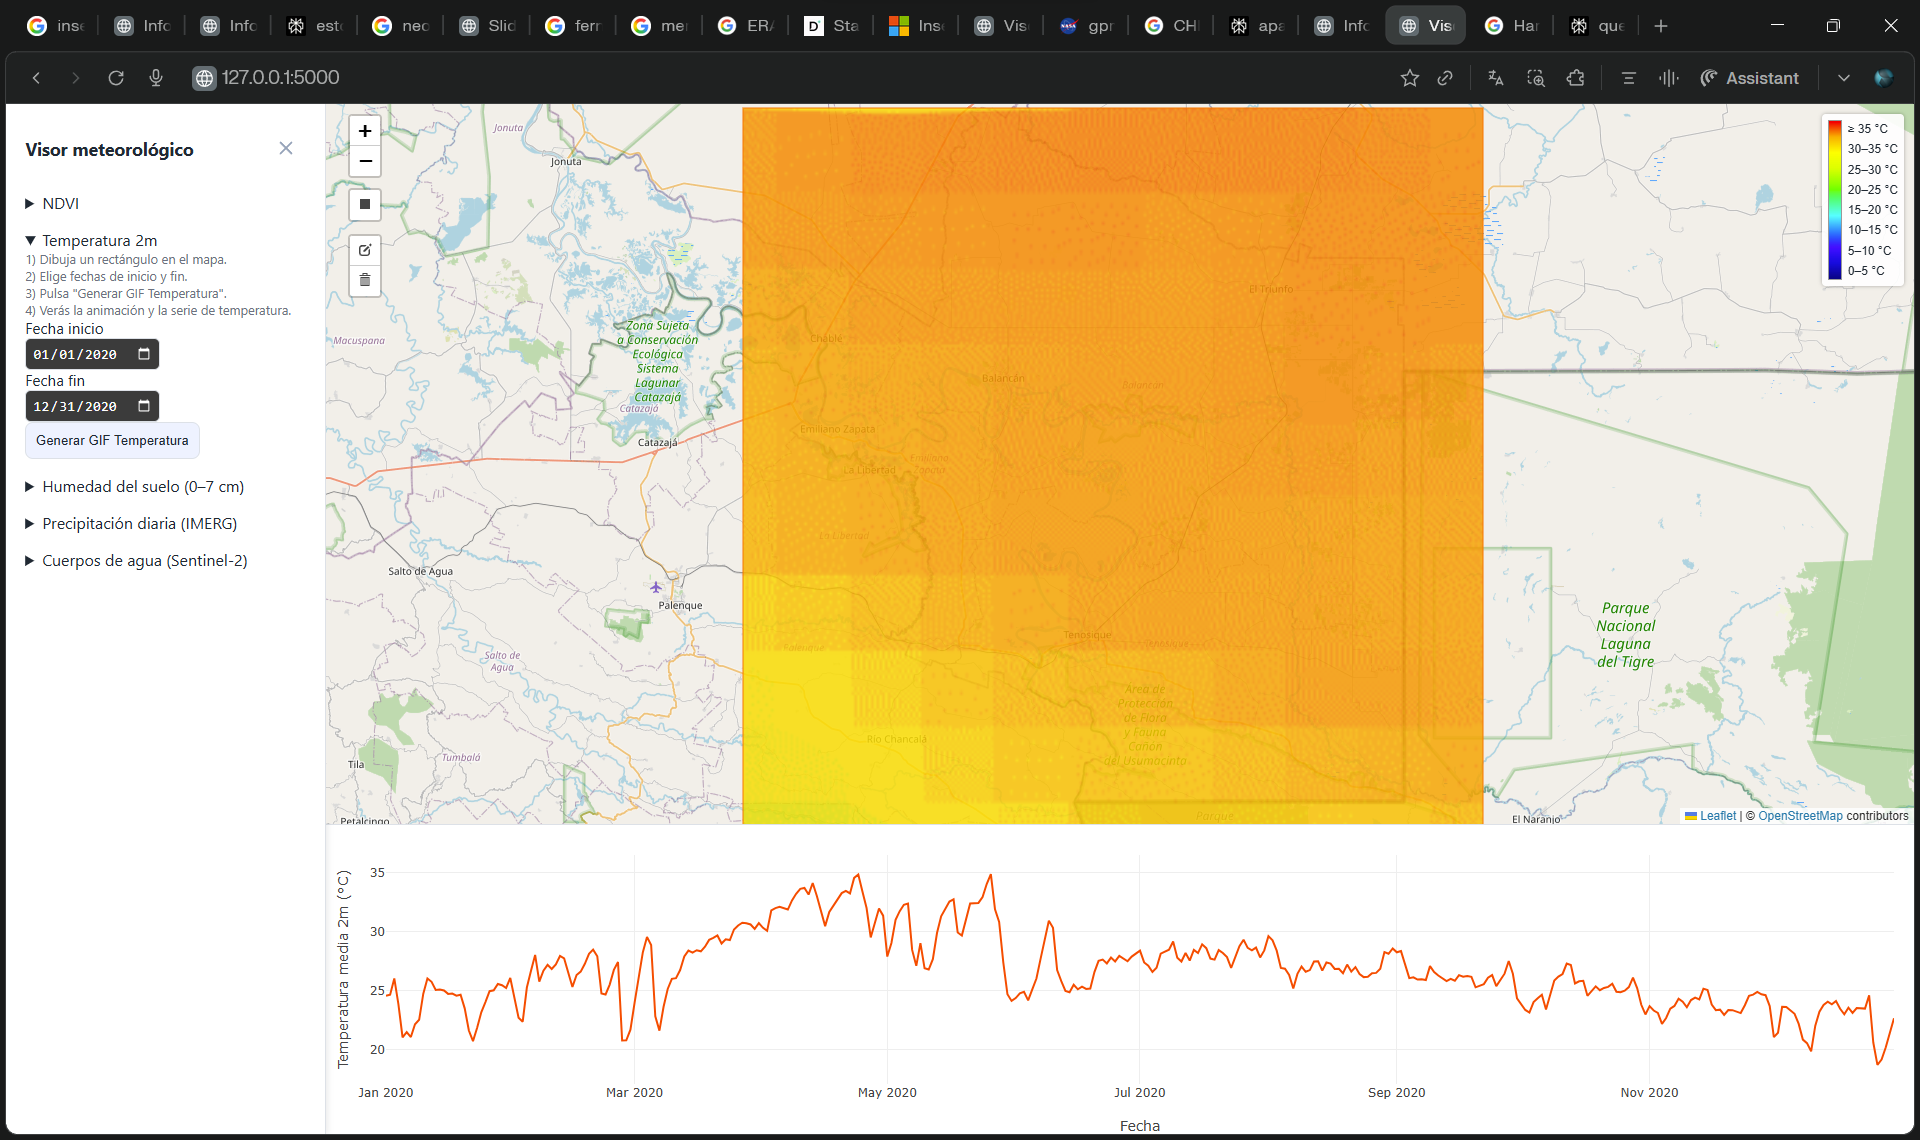
\includegraphics{21-ejemplo-temperatura.png}}

\end{center}

\end{frame}



\begin{frame}{Ejemplo: Análisis de Humedad del Suelo}

\begin{center}

% IMAGEN: Captura mostrando análisis de humedad del suelo:

% - GIF de humedad del suelo

% - Gráfica de serie temporal de humedad del suelo

% - Barra de colores de humedad del suelo

\resizebox{0.75\textwidth}{!}{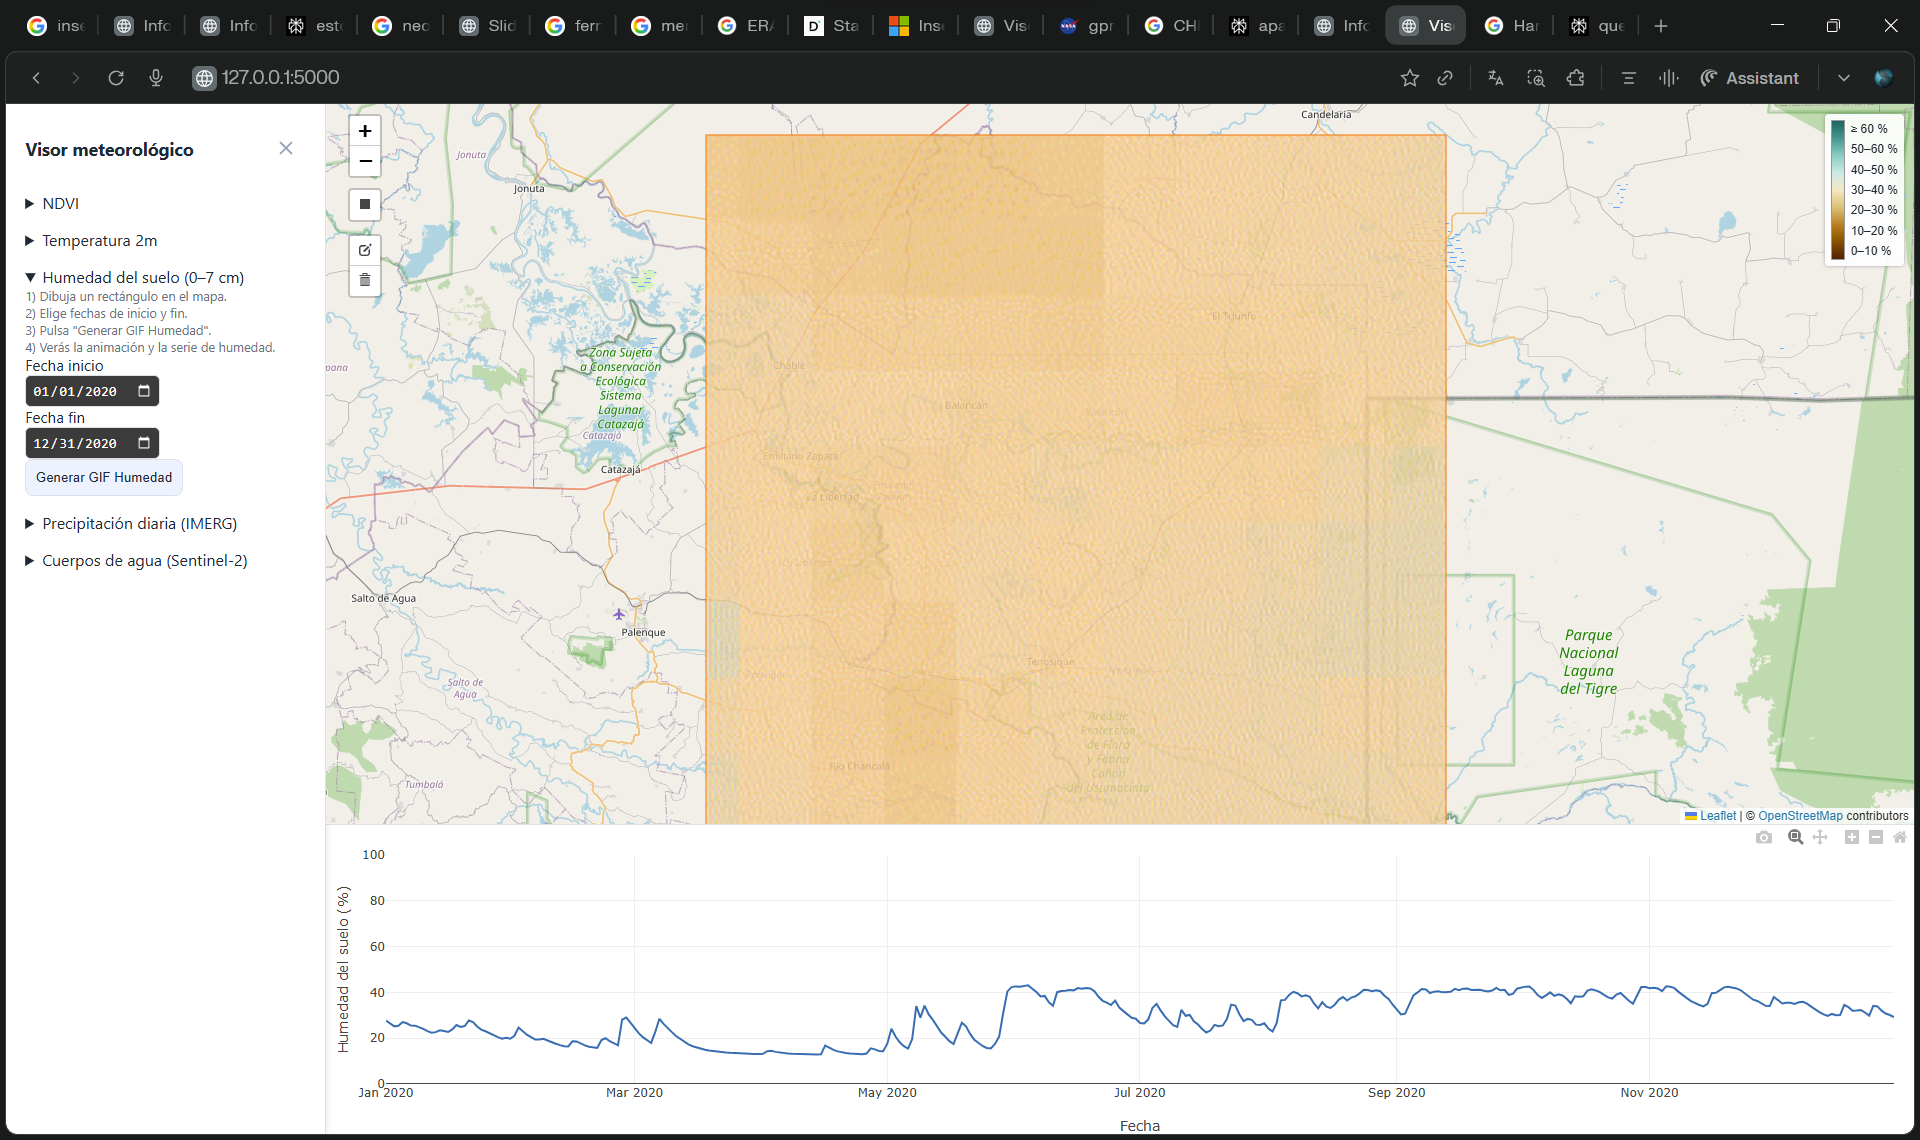
\includegraphics{29-ejemplo-humedad-suelo.png}}

\end{center}

\end{frame}



\begin{frame}{Ejemplo: Análisis de Precipitación}

\begin{center}

% IMAGEN: Captura mostrando análisis de precipitación:

% - GIF de precipitación

% - Gráfica de serie temporal de precipitación

% - Barra de colores de precipitación

\resizebox{0.75\textwidth}{!}{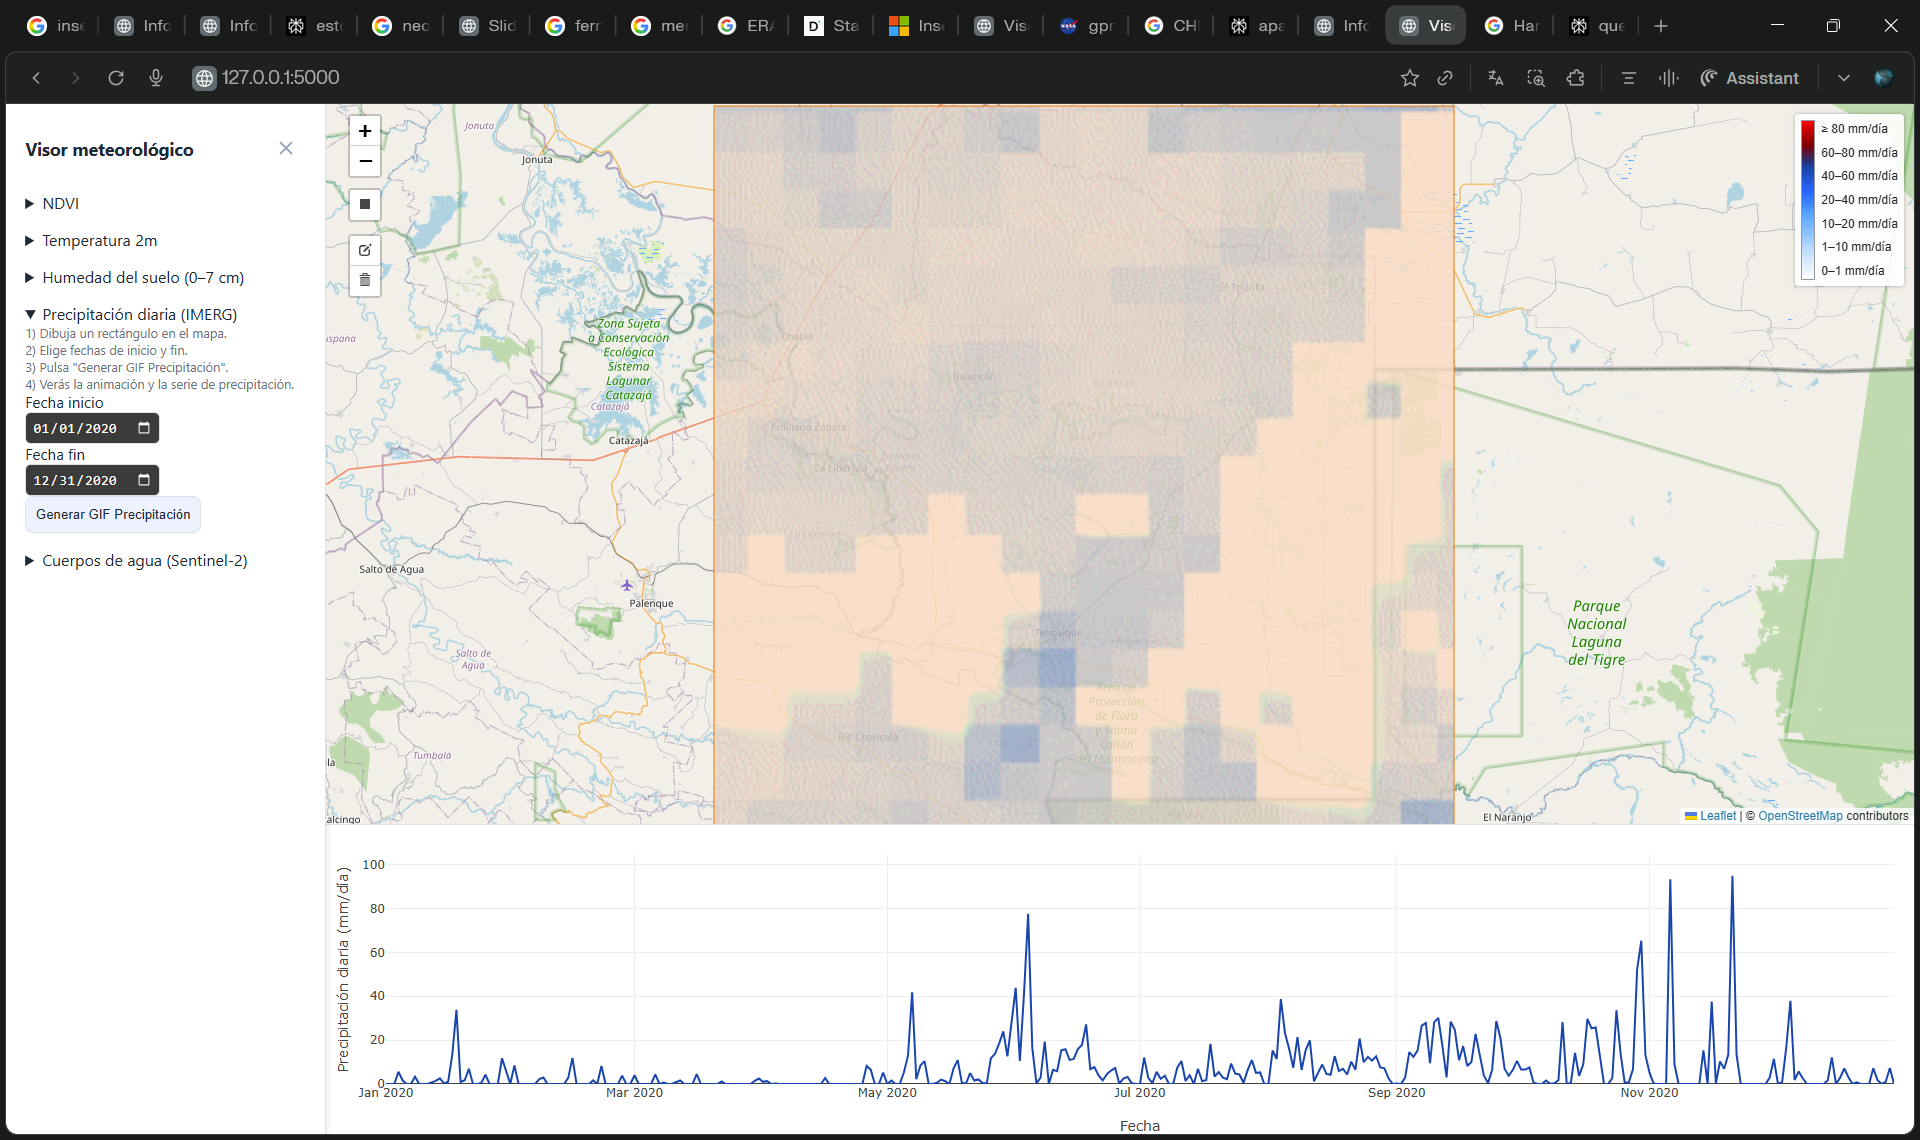
\includegraphics{30-ejemplo-precipitacion.png}}

\end{center}

\end{frame}



\begin{frame}{Ejemplo: Análisis de Agua Superficial}

\begin{center}

% IMAGEN: Captura mostrando análisis de agua superficial:

% - GIF de agua superficial

% - Gráfica de serie temporal de agua superficial

% - Barra de colores de agua superficial

\resizebox{0.75\textwidth}{!}{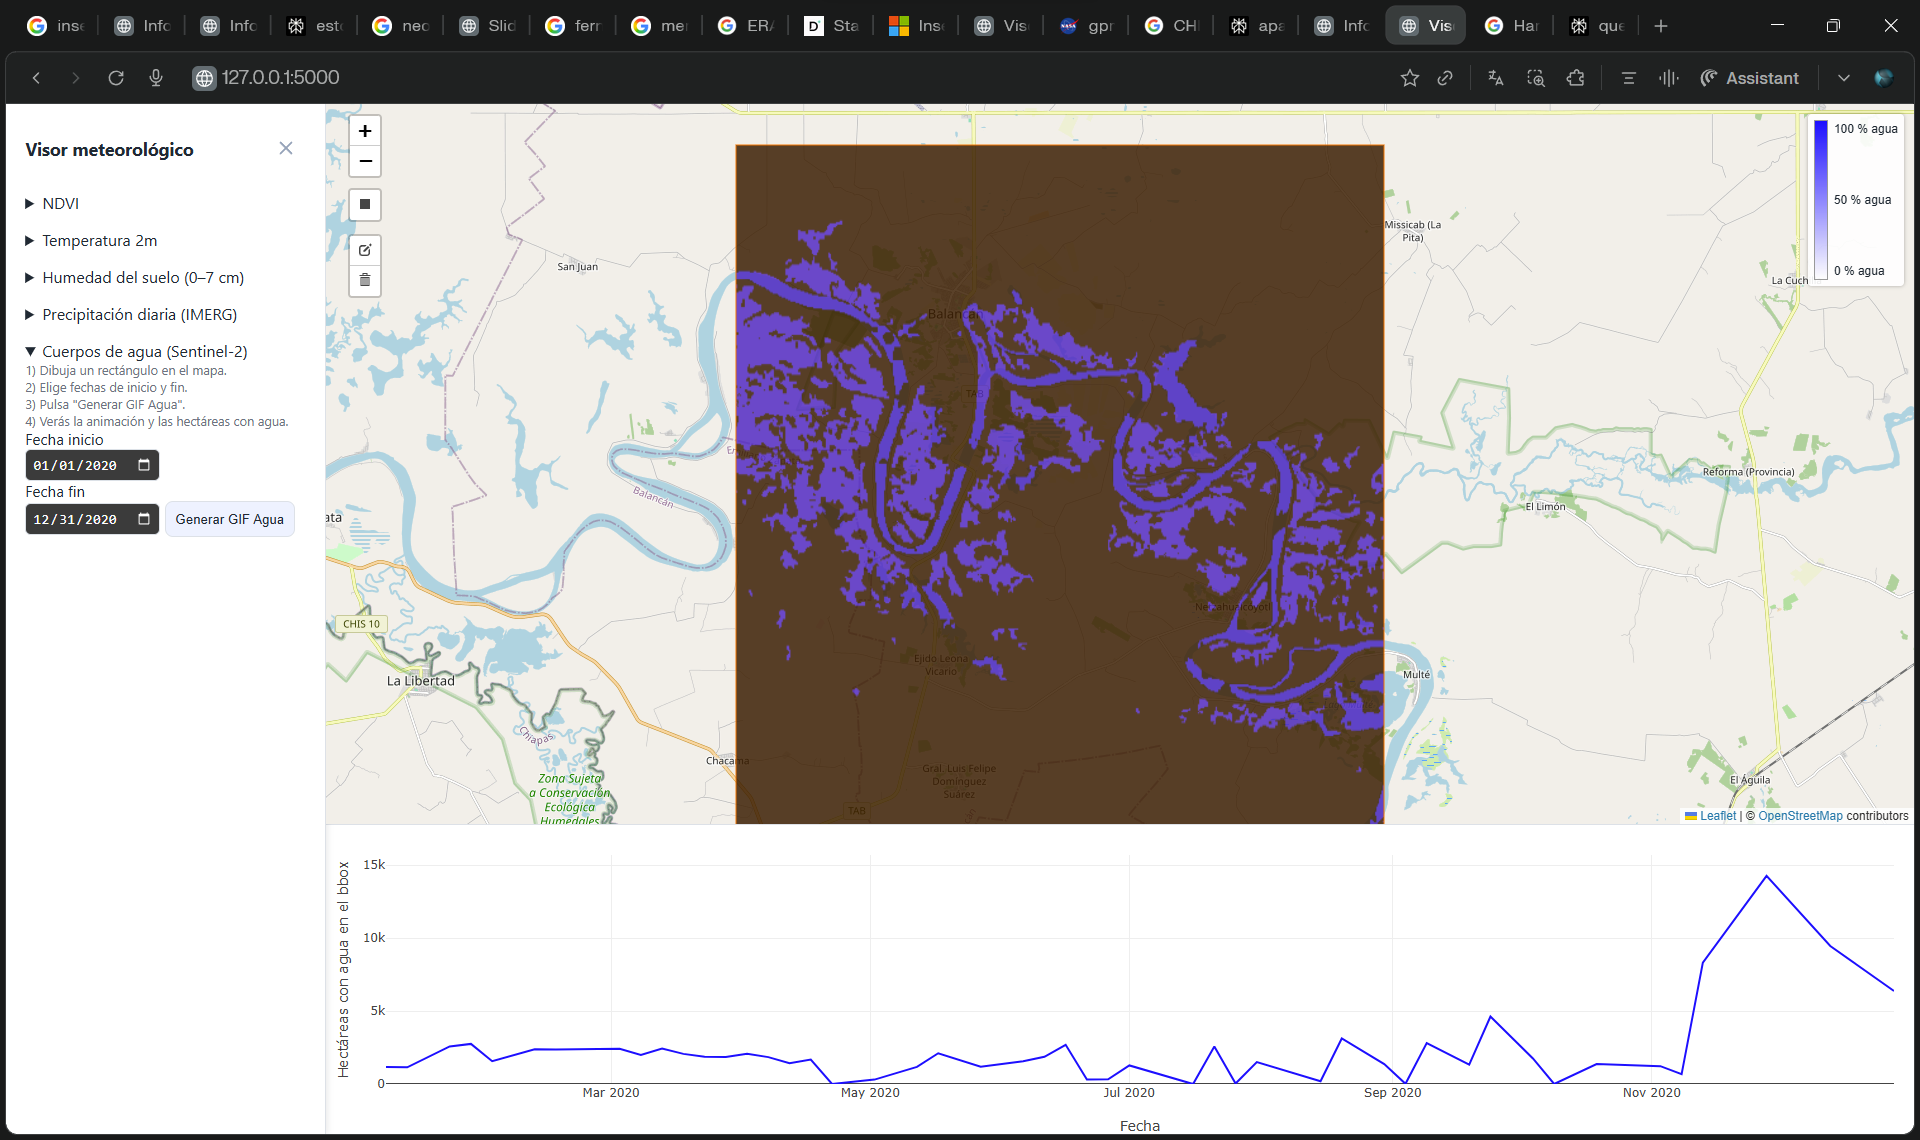
\includegraphics{31-ejemplo-agua-superficial.png}}

\end{center}

\end{frame}

% ============================================

% SECCIÓN 10: TRABAJO FUTURO

% ============================================

\section{Trabajo Futuro}



\begin{frame}{Mejoras Planificadas}

\begin{center}

% IMAGEN: Roadmap visual o diagrama de mejoras futuras

%\includegraphics[width=0.8\textwidth]{25-mejoras-futuras.png}

\end{center}

\begin{itemize}

\item Más variables meteorológicas

\item Exportación de datos

\item Comparación de períodos

\item Mapa de riesgos

\item Mejoras en la interfaz

\end{itemize}

\end{frame}



% ============================================

% CONCLUSIÓN

% ============================================

\begin{frame}{Conclusiones}
\justifying
La aplicacion desarrollada facilita el acceso al análisis hidrometeorológico mediante la integración efectiva de Google Earth Engine, Flask y Leaflet, eliminando barreras técnicas y costosas para procesar datos satelitales de NDVI, temperatura, humedad, precipitación y agua superficial. La aplicación facilita la toma de decisiones informadas en agricultura, gestión de recursos hídricos y prevención de desastres naturales, haciendo accesible tecnología satelital avanzada a profesionales y estudiantes. El trabajo futuro se enfocará en incorporar variables adicionales como viento y presión atmosférica, desarrollar modelos predictivos de sequías e inundaciones, integrar datos de estaciones meteorológicas locales y optimizar la plataforma para dispositivos móviles, ampliando así su impacto y utilidad en la sociedad.

\end{frame}



\end{document}

